\documentclass[a4paper,10pt,twoside,openright]{report}
\addtolength{\oddsidemargin}{-.5in}
\addtolength{\evensidemargin}{-.5in}
\addtolength{\textwidth}{3cm}
\addtolength{\topmargin}{-.875in}
\addtolength{\textheight}{1.75in}
% \textwidth 16.59cm
% \textheight 21.94cm

\usepackage{amsmath}
\usepackage{lscape}
\usepackage{graphicx}
\usepackage[margin=0pt,font=small,labelfont=bf,labelsep=endash]{caption}
\usepackage{pdfpages}
\usepackage{amssymb}
\usepackage[position=t,singlelinecheck=off]{subcaption}
\usepackage{amsthm}
\usepackage{rotating}
\include{qcircuit} % Package used for typesetting quantum circuits. Included in directory
\usepackage{sectsty}
\usepackage[numbers,sort&compress]{natbib} % Natbib package, supports more fancy ways of citing
\usepackage{bm} %Allows for boldface of Greek characters in math mode.
\usepackage{placeins}
% \usepackage{layouts} %Used to print page-widths
\usepackage{tikz} %For drawing figures. Might make compilation slow.
\sectionfont{\sffamily\Large}
\subsectionfont{\sffamily}
\usepackage[Bjornstrup]{fncychap}
\ChTitleVar{\raggedleft\LARGE\sffamily\bfseries}
\ChNumVar{\fontsize{76}{80}\usefont{OT1}{phv}{m}{n}\selectfont}
%%%\setlength{\parindent}{0in}
\newcommand{\comment}[1]{} %Creates a command that does nothing in order to allow in-line comments

\setlength{\marginparwidth}{0pt}
\hfuzz=10pt %disables warnings for overfull hbox upto 10pt. Used for chapter headings
% \pdfsuppresswarningpagegroup=1 % Disables warnings for multiple pdfs with grouping on same page
\usepackage{fancyhdr}
\usepackage{hyperref} %Adds hyperlinks to references
\hypersetup{
    % bookmarks=false,         % show bookmarks bar?
    unicode=false,          % non-Latin characters in Acrobat’s bookmarks
    pdftoolbar=true,        % show Acrobat’s toolbar?
    pdfmenubar=true,        % show Acrobat’s menu?
    pdffitwindow=false,     % window fit to page when opened
    pdfstartview={FitH},    % fits the width of the page to the window
    pdftitle={Entanglement of Weakly-coupled Carbon-spins in Diamond},    % title
    pdfauthor={M.A. Rol},     % author
    pdfsubject={Quantum Computation},   % subject of the document
    pdfcreator={Adobe},   % creator of the document
    pdfproducer={M.A.Rol}, % producer of the document
    pdfkeywords={Entanglement} {Quantum computing} {Interference}{Parity Measurements}{Quantum Error Correction}, % list of keywords
    pdfnewwindow=true,      % links in new window
    colorlinks=true,       % false: boxed links; true: colored links
    linkcolor=darkgray,          % color of internal links
    citecolor=darkgray,        % color of links to bibliography
    filecolor=magenta,      % color of file links
    urlcolor=darkgray           % color of external links
}
\usepackage{enumerate}
\usepackage{cleveref} %Adds the cref command for clever referencing
% \usepackage{svg}

\begin{document}

\newenvironment{changemargin}[2]{%
\begin{list}{}{%
\setlength{\topsep}{0pt}%
\setlength{\leftmargin}{#1}%
\setlength{\rightmargin}{#2}%
\setlength{\listparindent}{\parindent}%
\setlength{\itemindent}{\parindent}%
\setlength{\parsep}{\parskip}%
}%
\item[]}{\end{list}}

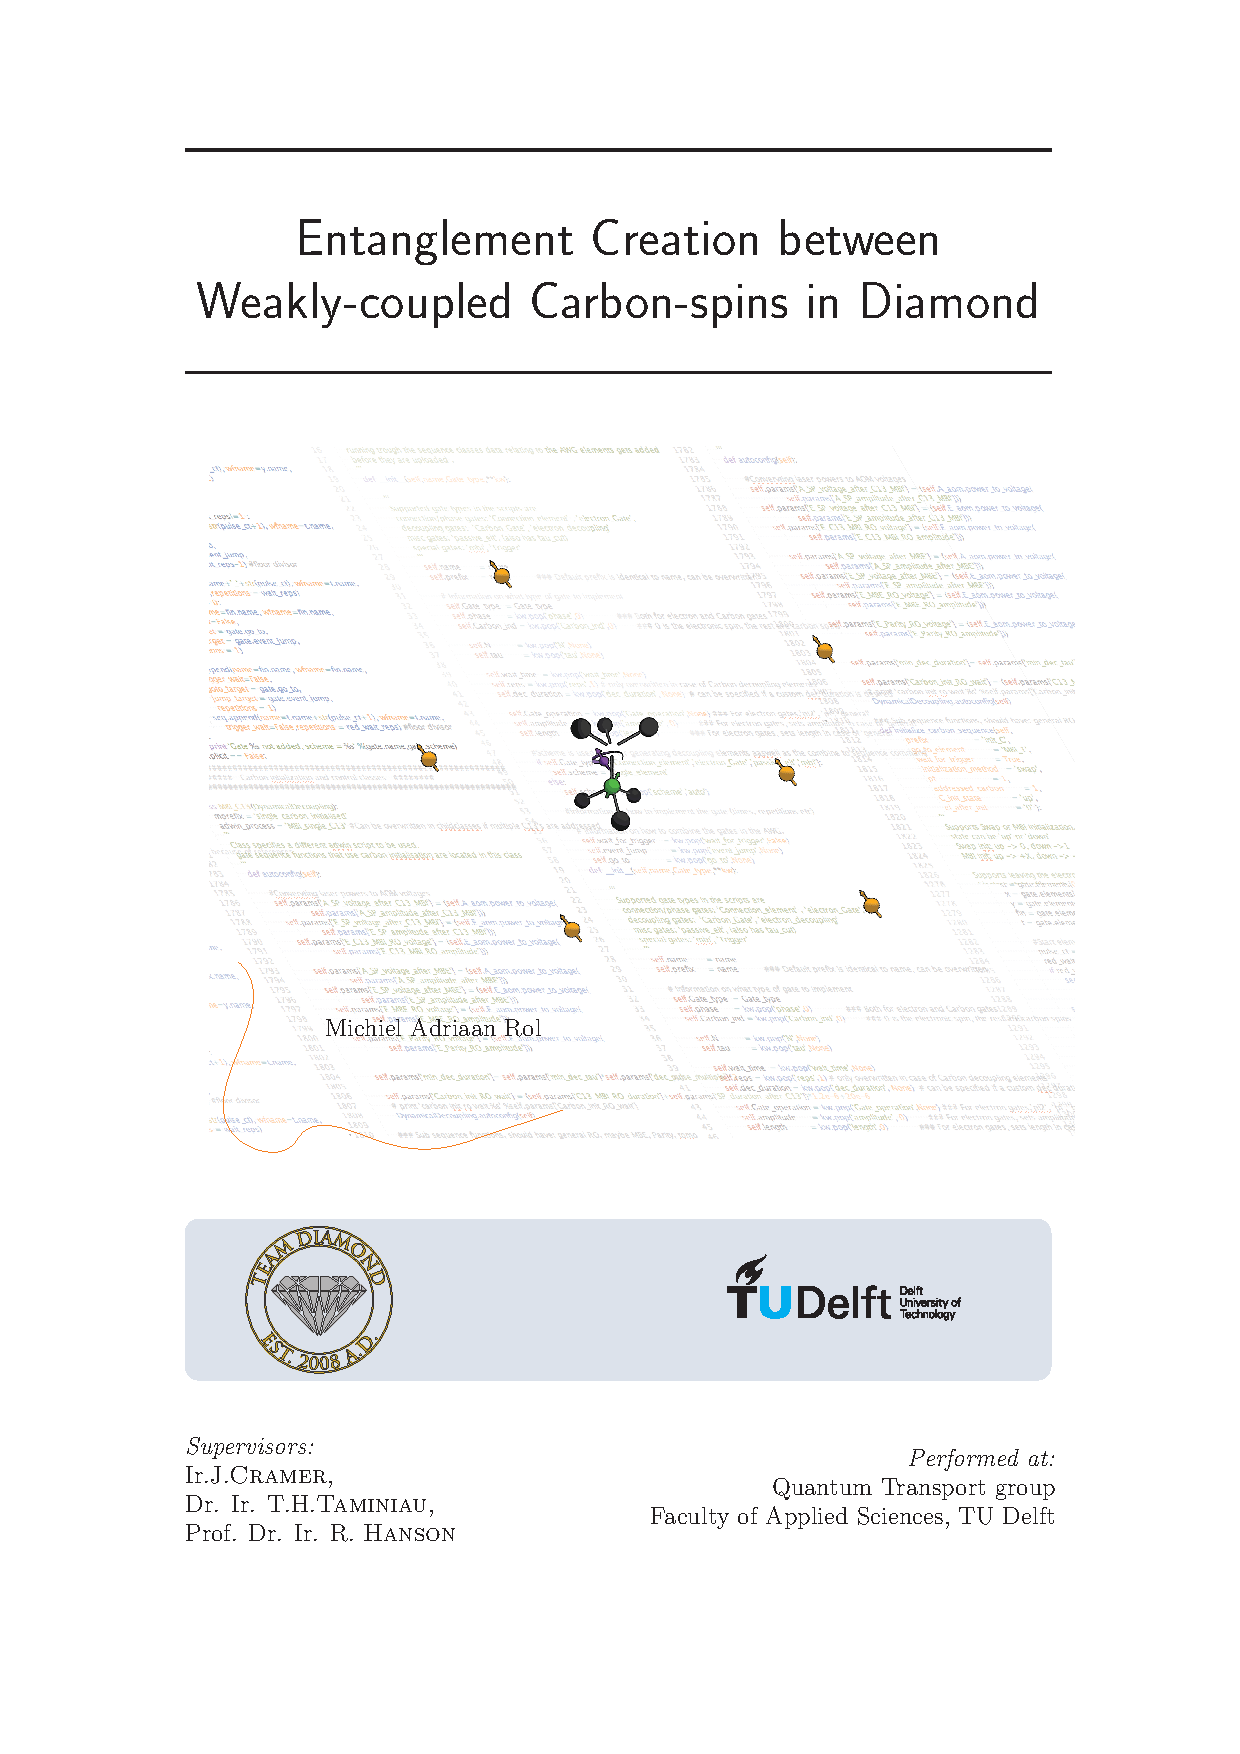
\includepdf{./Cover/cover_file.pdf}
\newpage
\thispagestyle{empty}
\mbox{}
\newpage

\begin{abstract}
Write Abstract here
\end{abstract}

\tableofcontents

\chapter{Introduction}
Although computers have increasingly become part of daily life they fall short when confronted with difficult problems  such as protein folding or searching a large unsorted database.
Quantum computers promise an exponential speedup for certain classes of problems making it possible to solve these problems on a human timescale.

A key challenge in building a large scale quantum computer is the presence of quantum errors.
To correct for these errors parity



% Qauntum computation is cool
% Hurdle Errors -> error correction
% System of choice NV center
% Goal of project

%weakly coupled carbons in NV- environment provide a naturally occuring spin register making it a promising candidate for QC
% For large scale larger and  deterministically available spin registers are desirable
% here we show deterministic generation of entanglement paving the way for measurement based QEC.
%  Simultations indicate that it is possible to control even more Carbon atoms extending the register and performing full QEC

% An essential feature for a scalable quantum computer is the ability to correct for quantum errors.
% The Nitrogen-Vacancy center in diamond is a promising candidate for a scalable quantum computer.
% In order to perform

% This chapter will explain why building a quantum computer is cool/important/essential/someotherbigword
% Explain why quantum error correction is essential in achieving this goal
% Requirements to perform quantum error correction
% Explain NV natural candidate
% Requirements 3-5 qubits + entanglement.
% This thesis will demonstrate how to address weakly coupled carbon spins and create entanglement between them.

% Paragraph: Quantum is cool because exponential scale up allowing previously unattainable problems

%The Nitrogen-Vacancy (NV) center in diamond is a promising candidate for a scalable quantum computer.
% An essential feature for building a scalable quantum computer is the ability to correct quantum errors.
% A basic form of Quantum Error Correction (QEC)  (cite references, either in NV or global)
% A logical next step is to perform QEC based on repeated parity measurements. (needs clarification).
% In order to perform measurement based QEC one needs to be able to initialize, control, read-out and entangle up-to 5 qubits.

\section{Quantum Computing}
The idea of using a quantum mechanical system to simulate physics was first explored by Feynman\cite{Feynman1982Simulating}.
Because the number of operations required to simulate a quantum system scales exponentially with the number of particles in the system it is not feasible to classically simulate such a system.
By manipulating a quantum mechanical system directly this scaling problem can be circumvented.

It was the idea of quantum simulation that led to the idea of exploiting quantum effects to perform computations.
Shor's algorithm \citep{Shor1994Algorithms} is a prime example of how the advantageous scaling of quantum systems can be exploited toe perform more efficient computations.

Shor's algorithm is an algorithm for prime factorization, where the best known classical algorithms for prime factorization scale exponentially Shor's algorithm scales polynomially.
Because of  the speedup provided by Shor's and other quantum algorithms it is possible to solve classes of problems that were previously unsolvable, such as the breaking of RSA encryption that relies on prime factorization being a computationally hard problem.
%Look up TJ Ladd et al. 2010 nature. On exponential speedup and entanglement as key resource. Can I link entanglement as resource to the propagation of errors?
% Proof of concept exists (+ examples of basic algorithms) but key challenge is scaling it up
Shor's algorithm has been shown to work on a small scale quantum computer \cite{Vandersypen2001Experimental}.
However to take full advantage of the efficient scaling behaviour of quantum computations a scalable quantum computer is required.

\section{Quantum Error Correction}
One of the main challenges in creating a scalable quantum computer is the effect of errors.
Because a quantum computer uses entanglement between multiple qubits as a resource an error an a single qubit can quickly propagate trough the system.
Using quantum error correction (QEC) it is possible to correct for such errors.
The threshold theorem states the final error probability of a quantum algorithm on a large register can be made arbitrarily small, if the probability of an error on a single qubit is below a certain threshold and QEC is applied \citep{Mermin1990Extreme}.
This makes quantum error correction a stepping stone on the way to realizing a scalable quantum computer \citep{Nielsen2010Quantum}.

Experiments demonstrating a form of QEC have been demonstrated in a range of systems.
Codes correcting for one type of quantum error have been implemented with nuclear magentic resonance \citep{Cory1998Experimental,Moussa2011Demonstration}, trapped ions \citep{Schindler2011Experimental}  and superconducting qubits \citep{Reed2012Realization}.
Recently two groups have implemented three qubit gate based QEC using the nitrogen-vacancy (NV) center in diamond \citep{Taminiau2014Universal,Waldherr2014Quantum}.

Although schemes exist to implement a scalable quantum computer using a purely gate based architecture most approaches rely on correcting for quantum errors by performing repeated parity measurements. An example of such an approach is surface coding \citep{Fowler2012Surface}.
For this reason the present work will focus on performing the parity measurements required for such error correcting schemes.

QEC is similar to classical error correction trough majority voting.
In classical majority voting a single bit is encoded onto a \emph{logical} bit consisting of multiple regular bits.
When an error on a bit has occurred the original bit can be recovered by measuring all the individual bits and determining the original state by majority voting.

In QEC the quantum bit (qubit) is encoded onto a logical qubit consisting of multiple regular qubits.
A consequence of classical majority voting is that it destroys a quantum state because it requires all bits to be measured.
By measuring the parity of two qubits the difference between two states can be determined without measuring the individual states.
If two states are parallel in the parity basis the parity measurement will return a positive result, if they are anti-parallel a negative result.
Performing a parity measurement on multiple qubits allows quantum errors, such as a bit-flip, a phase-flip or the combination of both, to be diagnosed.

\Cref{fig:gate_circuit_3_qubit_QEC} shows a circuit diagram for three qubit measurement based QEC.
The state $\ket{\psi}_\mathrm{C2}$ is encoded onto a logical qubit consisting of qubits C1, C2 and C3.
A parity measurement is performed on qubits C1 and C2, and on C2 and C3,  by reading out an ancilla qubit $e$.
From the result of the parity measurements it can be determined on which qubit an error occurred.
Based on this result the error can be corrected.
Because the logical qubit does not need to be decoded to correct for the error it is possible to repeat the error correcting part of the circuit, thereby improving the protection of the qubit.
The original qubit can be recovered by decoding the logical qubit.

\begin{figure}[htbp]
    \centering
    \mbox{
    \Qcircuit @C=1em @R=.7em {
        &&&& \control &\cw & \cw &\cw & \cw &\cw & \cw &\cw & \control \cw &\\
        \lstick{\ket{0}_e }        & \qw & \targ &\targ & \meter \cwx &  && \lstick{\ket{0}_e}     &\qw & \targ & \targ & \meter &  \cw \cwx  &\lstick{\ket{0}_e} &\qw&\qw &\qw &\rstick{\ket{0}_e} \\
        \lstick{\ket{0}_{\mathrm{C1}}}     &  \targ \qwx[1]& \ctrl{-1} &\qw & \qw &\qw&\qw& \qw &\qw & \qw &\qw & \qw & \multigate{2}{\mathrm{Corr.}} \cwx &\qw &\qw &  \targ \qwx[1] &\qw &\rstick{\ket{0}_{\mathrm{C1}}}\\
        \lstick{\ket{\psi}_{\mathrm{C2}}} &  \ctrl{1} & \qw &\ctrl{-2} & \qw &\qw&\qw&\qw  & \qw&\ctrl{-2} &\qw &\qw &\ghost{\mathrm{Corr.}}&\qw & \qw  &  \ctrl{1}&\qw &\rstick{\ket{\psi}_{\mathrm{C2}}}\\
        \lstick{\ket{0}_{\mathrm{C3}}}     & \targ   &\qw &\qw& \qw &\qw&\qw& \qw &\qw & \qw &\ctrl{-3} & \qw &\ghost{\mathrm{Corr.}}& \qw &\qw &  \targ&\qw &\rstick{\ket{0}_{\mathrm{C3}}}
        \gategroup{1}{3}{5}{13}{.7em}{--}  \
        % \gategroup{1}{3}{5}{12}{.7em}{_\}}
        % \gategroup{1}{13}{5}{13}{.7em}{_\}}
        % \gategroup{1}{1}{5}{2}{.7em}{_\}}
        % \gategroup{1}{14}{5}{14}{.7em}{_\}}
        }
    }
    \caption{Gate circuit for three qubit error correction. First the state of $C2$ is encoded onto three qubits.
    To diagnose an error an ancilla qubit is used to perform two parity measurements on the encoded qubits.
    The result of these measurements is used to determine what gates to apply to correct for the error if it occurred.
    These error correcting operations (in the dahsed lines) can be repeated to continuously protect the encoded qubits against quantum errors.
    The three qubit error correction code can correct for one type of quantum error. }
    \label{fig:gate_circuit_3_qubit_QEC}
\end{figure}

In order to implement measurement based error correction as depicted in \cref{fig:gate_circuit_3_qubit_QEC} we require initialization and control over three qubits and an ancilla that can be used to read out the main qubits.
Furthermore we need to be able to perform parity measurements on these qubits and deterministically perform operations based on the outcome of these parity measurements to correct for errors.

\section{The Nitrogen Vacancy Center in Diamond}
The NV-center is a promising candidate for quantum computation \citep{Childress2013Diamond}.
The NV-center is a naturally occurring impurity in diamond of which the electronic spin can be optically addressed and read out.
By applying microwave pulses to the NV-center it is possible to control and initialize strongly coupled spins in its environment \citep{Robledo2011HighFidelity}.
This spin register can be extended by addressing weakly coupled spins \citep{Taminiau2014Universal,Waldherr2014Quantum}.

Because of optical interface of the NV-center it is possible to link physically independent NV-centers together \citep{Bernien2013Heralded}. This has been used to demonstrate quantum teleportation \citep{Pfaff2014Unconditional}.

This unique combination of a local qubit register with an optical interface makes the NV-center a suitable system to implement a node based design for a scalable quantum computer\citep{Nickerson2013Topological}.

\section{Goal of the project}
In order to realize QEC at least three qubits are required to correct for a single type of error and more than five qubits are required to correct for a universal error.
Because the probability of finding enough strongly coupled carbons to implement QEC is small and goes down rapidly the more spins are required \citep{Waldherr2014Quantum,Taminiau2014Universal} we address weakly coupled spins using the methods developed by \citet{Taminiau2014Universal}.

The goal of this project is to implement  a parity measurement and demonstrate entanglement created by this parity measurement using weakly coupled spins in the environment of the NV-center.
The parity measurement is required for QEC in particular and measurement based approaches to quantum information in general.
This is done in a measurement environment that is designed from start to be compatible with the feed forward operations required for QEC.

The next chapter will explain the tools available to control the NV-center and strongly coupled spins.
\Cref{chap:addressing_weakly_coupled_carbons} will discuss how coherence can be extended
in order to control weakly coupled carbons.
In \cref{chap:control_weakly_carbon} these techniques are used to first initialize multiple weakly coupled carbon spins before creating entanglement using the parity measurement.
The last chapter will provide an outlook on how the capabilities developed can be extended to perform deterministic parity measurements and show simulations indicating that it is possible to perform multi qubit error correction using weakly coupled spins.

% Gives motivation for doing parity measurements based on the importance of QEC
% Clearly ending in several key requirements for the experiments:
        %  Control of enough qubits /carbons
        %  Feed forward -> Deterministic gates and dynamical operations
        %  Parity measurements
\chapter{The Nitrogen-Vacancy center in Diamond}
The nitrogen-vacancy (NV) center in diamond provides a natural occurring qubit register in a solid state environment.
This chapter will explain how the electronic spin can be initialized, controlled and read-out using optical and microwave pulses.
The electronic spin can be used to initialize control and readout nuclear spins in the environment trough the hyperfine interaction.
It is shown how the coherence of the electron poses challenges to directly control the nuclear spin.
The next chapter will demonstrate how to extend the electron coherence so that more spins can be controlled.

\section{The Electronic Spin}
The NV-center is a naturally occurring impurity in diamond consisting of a substitutional nitrogen and an adjacent lattice vacancy (\cref{fig:Sil_Robledo}).
The NV-center can be in a neutral charge state ($\mathrm{NV}^0$) or in a negatively charged state ($\mathrm{NV}^-$).
In this thesis we are mainly interested in the negatively charged state, where an additional electron is captured from the environment.
For the $\mathrm{NV}^-$ the ground state is a spin-triplet that forms the basis of our qubit.

The electronic ground state can be described by the Hamiltonian \citep{Bernien2014Control}:
 \begin{equation}
H_\mathrm{GS} = \Delta {{S}_\mathrm{z}}^2 + \gamma_e \bm{B} \cdot \bm{S}
\end{equation}
Where $\bm{S}_i$ are the Pauli-spin operators,  $\gamma_e  = 2.802\,\mathrm{ MHz/G}$  is the electron gyro-magnetic ratio and $\Delta \approx 2.88\, \mathrm{GHz}$ is the zero-field splitting.
In this expression the interactions with the nitrogen nucleus and the carbon spin bath are not included.
In the experiments a magnetic field $B_z = 304\,\mathrm{G}$ is applied along the NV-axis\footnote{The NV-axis is the axis going trough both the nitrogen and the vacancy. }.
The magnetic field lifts the degeneracy of the $m_s = \pm 1$ so that we can define our electronic qubit  as the two level system  $m_s=0:=|0\rangle$ and $m_s = +1 := |1\rangle$.

\begin{figure}[htbp]
    \centering
    \begin{subfigure}[t]{0.49\textwidth}\centering
        \caption{}
        \label{fig:Sil_Robledo}
        \includegraphics[scale = 1.4]{Img/Sil_Robledo.pdf}
    \end{subfigure}
    \begin{subfigure}[t]{0.49\textwidth}\centering
       \caption{}
       \label{fig:readoutRobledo}
       \includegraphics[scale = 1.4]{Img/readout_Robledo.pdf}
   \end{subfigure}
   \caption{\textbf{\subref{fig:Sil_Robledo}} Scanning electron microscope image of a diamond sample with solid immersion lens (SIL) similar to that used in the experiments.
   A gold stripline, visible as the white area below the SIL is used to apply microwave pulses.
   Overlaid sketch shows a schematic representation of the NV-center. Inset shows a confocal microscope image of the NV-center in the center of the SIL. \textbf{\subref{fig:readoutRobledo}}, Energy levels used for initialization and readout of the electronic-spin state. Figures adapted from \citet{Robledo2011HighFidelity}}
\end{figure}

\subsection{Initialization and readout of the electronic-spin state}
The transitions between the electronic ground-state and excited state are spin dependent and lie in the optical domain ($\sim 637\, \mathrm{ nm}$).
At low temperatures these transitions can be resonantly excited.
For this reason, experiments were performed at cryogenic temperatures ($4\,\mathrm{K}$).
The exact frequencies of these transitions depend on magnetic field and strain \citep{Hensen2011MeasurementBased}.

\Cref{fig:readoutRobledo} shows the optical transitions used to initialize and read-out the electronic spin.
The $E'$ transition excites both the $m_s =+1$ and the $m_s=-1$ states to the excited state.
The $E_\mathrm{x}$ transition excites the $m_s = 0$ state to the excited state.
There is a small probability that the spin is flipped in an optical cycle, denoted by the dashed line.

By cycling an optical transition the spin state can be read-out and initialized \citep{Robledo2011HighFidelity}.
By applying a pulse to the $E_x$ transition a photon can be detected when the state falls back to the ground state.
Because the $E_x$ only excites the $m_s=0$ state photons can only be detected when the system is in the $\ket{0}$-state.

By pumping one of these transitions the spin can be initialized.
Pumping will cause the population to cycle between the ground and excited state with a small probability of the spin flipping.
When the spin flips it ends up in the state that is not being excited and stays there.

Because the number of pumping cycles before the spin flips is limited, the fidelity with which the spin can be read-out is limited by the detection efficiency of the emitted photons.
A solid immersion lens (SIL), visible in \cref{fig:Sil_Robledo}, is milled onto the sample to maximize the detection efficiency.
The experiments in this thesis were performed at a readout fidelity of $F\approx 91\%$.

\subsection{Controlling the electronic-spin state}
The state of a qubit can be represented as a vector on the Bloch-sphere where the $\ket{0}$-state lies at the north pole and the $\ket{1}$-state at the south pole.
The state vector rotates around the quantization-axis with a frequency depending on the energy splitting between the two states: the Larmor frequency.
For the NV-electronic spin the quantization axis points in the z-direction (towards $\ket{0}$) and the  Larmor frequency is given by:
\begin{equation}
    \omega_L =\Delta + \gamma_e {B_\mathrm{z}}
    \label{eq:larmor_electronic_spin}
\end{equation}


By applying an external field a term is added to the Hamiltonian, the quantization-axis is changed, thereby changing its evolution.
By applying microwaves with a frequency equal to $\omega_L$ the transition between $\ket{0}$ and $\ket{1}$ can be driven \citep{Jelezko2004Observation}.
Resonant microwave pulses are applied to the sample trough an on-chip stripline (\cref{fig:Sil_Robledo}).

\section{Controlling Nuclear Spins}
The electronic-spin interacts with each nuclear spins in its environment trough the hyperfine interaction, which is dependent on their position.
Dependent on the strength of the hyperfine interaction close by spins can be controlled directly by applying microwave pulses.

\subsection{The Hyperfine Interaction}
The coupling between the electronic spin of the NV-center and a nuclear-spin is given by the hyperfine-interaction.
The hyperfine interaction is a spin-spin interaction.

For nuclear spins the Hamiltonian therefore depends on the electronic spin-state of the NV-center.
For a magnetic field ($B_\mathrm{z}$) in the z-direction the Hamiltonian is given by:
\begin{equation}
    \label{eq:nuclear_hamiltonian_0}
    H_0= -Q I_{\mathrm{z}}^2+ \gamma_{n} B_\mathrm{z} I_\mathrm{z}
\end{equation}
\begin{equation}
    \label{eq:nuclear_hamiltonian_1}
    H_1 = -Q I_{\mathrm{z}}^2+\gamma_{n} B_\mathrm{z} I_\mathrm{z} +H_{\mathrm{HF}}
\end{equation}
Corresponding respectively to the electronic spin being in the $m_s = 0$ and in the $m_s = +1$ state.
Where $\bm{I}$ and $\bm{S}$ are the nuclear and electronic spin operators, $\gamma_n$ is the gyro-magnetic ratio of the nucleus and $Q$ is the nuclear quadrupole splitting.
The quadrupole term is $Q= 2\pi \cdot 4.946 \,\mathrm{ MHz}$ for the nitrogen-14 spin \citep{Bernien2014Control}.
And $Q = 0$ for carbon-13 spins.


The Larmor frequency for a nucleus is given by  \cref{eq:nuclear_larmor}:
\begin{equation}
\label{eq:nuclear_larmor}
{\omega_L} =-Q{I}_{\mathrm{z}}^2+ \gamma_{n}B_\mathrm{z}
\end{equation}

\subsection{Controlling the nitrogen nuclear spin}
\label{sec:nitrogen_spin_control}
To obtain high-fidelity electron spin control it is desirable to initialize the nitrogen of the NV-center.
In this work this is done through measurement based initialization (MBI) using the hyperfine interaction.

Because both the zero-field splitting $\Delta$ of the electronic-spin is much larger than the hyperfine coupling between the nuclear and electronic spin, the secular approximation can be used, leading to the following system Hamiltonian:
\begin{equation}
        H_\mathrm{GS} = \Delta {{S}_\mathrm{z}}^2 + \gamma_e \bm{B} \cdot \bm{S} -Q I_{\mathrm{z}}^2+\gamma_{n} B_\mathrm{z} I_\mathrm{z} - A_\mathrm{N} S_z\cdot {I_z}
\end{equation}
Where $A_\mathrm{N} = 2\pi \cdot 2.186 \, \mathrm{MHz} $.
The hyperfine interaction between the nitrogen and electronic spin causes the transition between $m_s=0$ and $m_s =1$ to be split.
This magnitude of the splitting is equal to $A_N$ and  is clearly resolved in the Electron Spin Resonance (ESR) shown in the top panel of \cref{fig:HF_split_levels}.


    \begin{figure}[htbp]
    \centering
        \begin{tikzpicture}
            \node[anchor=south west,inner sep=0] at (0,0) {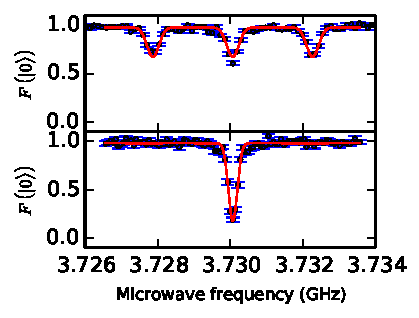
\includegraphics{Img/DarkESR_2.pdf}};
            \node (A) at (2.6,4.4) {};
            \node (B) at (3.92,4.4) { };
            \node (C) at (5.3,4.4) { };
            \draw[latex-latex, font=\small] (A) -- node[label =270: $A_\mathrm{N}$] {} (B);
            \draw[latex-latex, font=\small] (B) -- node[label =270: $A_\mathrm{N}$] {} (C);
        \end{tikzpicture}
        \caption{ Electron Spin Resonance (ESR) for uninitialized (top) and initialized nitrogen spin (bottom) of the $m_s =0 \rightarrow m_s = +1$ transition. In the ESR the spin is prepared in $\ket{0}$, a microwave pulse is applied and finally the electron spin fidelity with $\ket{0}$, $F(\ket{0} )$ is measured.
        The microwave frequency is swept.
        When the microwave is on resonance the spin will be rotated out of $\ket{0} $ and a decrease will be visible in the signal.
        In the top figure the transition is split due to the interaction with the NV's nitrogen nuclear spin.
        In the lower figure the nitrogen spin state is initialized and the splitting disappears.}
        \label{fig:HF_split_levels}
    \end{figure}

The hyperfine interaction can be used to measure the nitrogen's spin state.
Every time an experiment is started the nitrogen starts out in a mixed state.
This means that every time an uninitialized nitrogen is measured it is equally likely to end up in one of its three states, as can be seen in the top panel of \cref{fig:HF_split_levels}.
The nitrogen state can be measured by initializing the electron in the split $m_s = +1$ state and driving one of the transitions to $m_s=0$, factually implementing a controlled-NOT gate.
Only if the nitrogen was in the state corresponding to the transition being driven will a measurement of the $m_s =0$ state give a positive result.

By resetting and repeating this procedure until a positive result is measured the nitrogen-spin can be initialized.
The electronic spin-state can be reset by applying a resonant laser as shown in the previous section.
The nuclear spin-state can be reset by applying two resonant lasers resonant with $E_x$ and $E'$ to introduce electron-nuclear flip-flops.

This procedure is known as measurement based initialization (MBI) and is used in our experiments.
The lower panel of \cref{fig:HF_split_levels} shows an ESR after the nitrogen has been initialized using MBI.

\subsection{Hyperfine coupling of carbon-13 spins}
For carbon-13 spins the hyperfine term ($H_{\mathrm{HF}}$) of \cref{eq:nuclear_hamiltonian_1} consists of a contact term and a dipole term.
The contact term results from an overlap between the electronic- and nuclear- wave-functions.
The contact term is negligible for all but the carbon-spins closest to the NV-center.
For close-by carbon spins hyperfine couplings have been calculated \citep{Gali2008Ab,Gali2009Identification} and measured \citep{Smeltzer201113}.

For carbons where the contact term is negligible the dipole term is dominant and is given by \citep{Lange2012Quantum}:
\begin{equation}
\label{eq:dipole_component_of_hyperfine}
H_{\mathrm{dip}} = \frac{\mu_0 \gamma_e \gamma_{\mathrm{C}} \hbar^2 }{4 \pi r^3} [ \bm{S \cdot I} - 3 (\bm S \cdot \hat{\bm{n}}_{\mathrm{HF}})(\bm I \cdot \hat{\bm{n}}_{\mathrm{HF}})]
\end{equation}
Where $\hat{\bm{n}}_{\mathrm{HF}}$ is a unit vector pointing from the electronic spin to the nucleus, $r$ is the distance between the electronic and nuclear spin, and $\mu_0$ the magnetic constant.
The dipole term can be split into a parallel ($A_\parallel $) and orthogonal ($A_\perp$) component such that:
\begin{equation}
     H_{\mathrm{HF}} = A_\parallel I_\mathrm{z} + A_\perp I_x
 \end{equation}


From \cref{eq:dipole_component_of_hyperfine}  the parallel and orthogonal components of the hyperfine interaction, with respect to the NV-axis along the z-direction, can be derived to be:
 \begin{align}
A_\parallel= - \frac{\mu_0 \gamma_e \gamma_{\mathrm{C}} \hbar^2 }{4 \pi r^3} \left(3\cdot \frac{z^2}{r^2}-1\right)\\
 A_\perp =  -\frac{\mu_0 \gamma_e \gamma_{\mathrm{C}} \hbar^2 }{4 \pi r^3}\left( 3\cdot\frac{\sqrt{x^2+y^2}\cdot z}{r^2}\right)
\end{align}


\subsection{Weakly versus strongly coupled carbon spins}
Carbon spins can be controlled using the methods described in \cref{sec:nitrogen_spin_control} when it is possible to selectively address its spin-dependent transitions.
When two transitions can be resolved in an ESR they can be addressed by applying microwave pulses of the corresponding frequencies.
However if two transitions overlap in an ESR, applying a microwave pulse at the corresponding frequency will address both transitions.

Two transitions cannot be resolved when the splitting between them is smaller than the width of the transition.
The magnitude of the splitting is determined by the strength of the interaction and the broadening of the transitions is caused by decoherence.
We define a spin to be strongly coupled when it is possible to readily resolve it's transitions in an ESR experiment with negligible power broadening.
Conversely a spin is weakly coupled when it is not possible to readily resolve its transitions in an ESR.
\Cref{fig:coupling regimes} shows a schematic overview of the different coupling regimes.

As the presence of strongly coupled carbons close to the NV-center is governed by probability and the probability of getting 3-5 strongly coupled carbons is very low it is necessary to develop methods to address weakly coupled carbons.
The next chapter will demonstrate methods to extend the coherence time and address weakly coupled carbons, thereby enlarging the spin-register.

Before coherence can be extended to control weakly coupled spins it is neccesarry to understand what decoherence is and how it relates to the broadening of transitions.
The next section will explain decoherence and give an estimation for the hyperfine strength above which a spin is strongly coupled.

\begin{figure}[htbp]
\centering
    \begin{tikzpicture}
        \node[anchor=south west,inner sep=0] at (0,0) {\includegraphics[scale = 0.5]{Img/coupling_regimes.eps}};
        \node[font=\tiny] at (5,4) {$A \approx \frac{\sqrt{\ln{2}}}{\pi T_{2\mathrm{C}}^*}$};
        \node[font=\tiny] at (4,3.1) {$A\approx \frac{\sqrt{\ln{2}}}{\pi T_{2e}^*}$};
        \node[font=\small] at (3.8,1.9) {$\mathbb{I}$};
        \node[font=\small] at (4.75,1.2) {$\mathbb{II}$};
        \node[font=\small] at (5.6,0.5) {$\mathbb{III}$};
        %Help grid for drawing
        % \draw[help lines,xstep=1,ystep=1] (0,0) grid (7,5);
        % \foreach \x in {0,1,...,7} { \node [anchor=north] at (\x,0) {\x}; }
        % \foreach \y in {0,1,...,5} { \node [anchor=east] at (0,\y) {\y}; }
    \end{tikzpicture}
    \caption{ Schematic representation of different coupling regimes. Carbons in region $\mathbb{I} $ are in the strong coupling regime, transitions of these spins can be readily resolved and they can be controlled using the methods described in \cref{sec:nitrogen_spin_control}.
    In the weak coupling regime (region $\mathbb{II}$) carbon-spins are coupled more strongly to the NV-center than to the spin-bath but not strong enough to be readily resolvable in an ESR. Some of these spins can be controlled trough dynamical decoupling \citep{Taminiau2012Detection}.
    In the very-weak coupling regime (region $\mathbb{III}$) the coupling to the spin-bath is stronger than the coupling to the NV-center. These spins cannot presently be addressed.}
    \label{fig:coupling regimes}
\end{figure}

\section{Decoherence}
Whether a nuclear spin is weak or strongly coupled is set by the coherence time of the electron spin.
This section will explain decoherence as well as give an estimation for when a carbon spin is strongly coupled.

An ESR signal is broadened because the NV-center interacts with the spin bath in its environment.
The spin bath consists of spins that are coupled to the NV-center.
Just like the uninitialized nitrogen spin these are in a mixed state.
This means that for every iteration of an experiment the spin bath can have a different configuration.
These different configurations of the spin bath slightly shift the addressed electron transition causing the broadening of the transition.

\subsection{Decoherence time}
The variations in the spin-bath configuration can be measured with a Ramsey experiment.
In a Ramsey experiment (\cref{fig:Ramsey_gijs}) the electronic spin is brought into a superposition between the $\ket{0}$ and $\ket{1}$-state where it freely evolves for a time $\tau$.
Provided the coherent superpsition is preserved, a final pulse brings the state back into $\ket{0}$ where it is read out.

By applying a slight detuning to the rotating frame used to keep the phase fixed an oscillation can be seen in the signal (\cref{fig:electron_T2*}).
Due to the different spin-bath configurations the evolution frequency varies slightly between experiments, this causes the measured signal to decay as the different oscillations move out of phase with each other.
The decay is known as decoherence and the $1/e$-time of the decay is the decoherence time $T_2^*$.
For a Ramsey experiment the decay follows a Gaussian profile:
\begin{equation}
    F(\ket{0})(\tau) = e^{-(\tfrac{\tau}{T_{2}^*})^n}
    \label{eq:Ramsey_decay}
\end{equation}
Where $n =2$ for a Gaussian profile.
The $T_2^*$ of the NV-electron spin used in this thesis was measured to be $T_{2,e}^* = 4.54 \pm 14\, \mu\mathrm{s}$ with initialized nitrogen-spin.
The decay is consistent with a Gaussian profile: $n = 1.81 \pm 0.14$.

\begin{figure}[htbp]
    \centering
    \begin{subfigure}[t]{0.49\textwidth}\centering
        \caption{}
        \includegraphics{Img/Ramsey_Gijs.pdf}
        \label{fig:Ramsey_gijs}
    \end{subfigure}
    \begin{subfigure}[t]{0.49\textwidth}\centering
        \caption{}
        \includegraphics{Img/electron_T2star.pdf}
        \label{fig:electron_T2*}
    \end{subfigure}
        \caption{
        \textbf{\subref{fig:Ramsey_gijs}} schematic representation of a Ramsey experiment. Figure from \citet{Lange2012Quantum}.
        In a Ramsey experiment a qubit is brought into the $xy$-plane by a $\pi/2$-pulse where it evolves freely for a time $\tau$ before being subjected to a final $\pi/2$ pulse to read out its $x$-component.
        By applying a detuning ($\omega_d$) to the rotating frame the spin will pick up a phase $\phi = \omega_d \tau$ during free evolution.
        The final pulse will rotate the spin towards the poles depending on the phase picked up during free evolution.
        This manifests itself as an oscillation.
        Because the configuration of the spin-bath is slightly different between experiments the frequency of the oscillation will vary with each iteration.
        This variation in frequency between iterations will cause the oscillation to decay.
        \subref{fig:electron_T2*} Ramsey experiment for the electronic spin.
        The $y$-axis shows the fidelity ($F(\ket{0})$) of the measured state to the $\ket{0}$-state of the electronic spin.
        A $T_{2,e}^*$ of $4.54 \pm 0.14\, \mu\mathrm{s}$ was measured for the electronic spin. The decay follows a Gaussian profile within uncertainty $n = 1.81 \pm 0.14$. }
\end{figure}


\subsection{Relation between decoherence and transition broadening}
The decay in a Ramsey experiment is a measure for variations of the spin-bath in the time-domain while the broadening of transitions in an ESR is a measure for variations of the spin-bath in the frequency domain.
The decay of the Ramsey and the shape of the ESR for negligible power broadening are related trough a Fourier transform and described by:
\begin{equation}
    \mathcal{F} \{ K(\tau) \} =  C e^{-\tfrac{(2\pi \cdot f) ^2 \cdot T_{2e}^{*2}}{ 4}}
    \label{eq:ESR_dip_shape}
\end{equation}
Where $C$ is a normalization constant.
Because the decay of the Ramsey is Gaussian the shape of a transition in the ESR is also Gaussian.

Two identical Gaussians can be readily resolved when the separation between their maxima is larger than their full-width-half-maximum (FWHM).
The FWHM (in Hz) of the ESR is given by \cref{eq:FWHM}:
\begin{equation}
    \mathrm{FWHM} =  \frac{2\sqrt{\ln{2}}}{\pi T_{2e}^*}
    \label{eq:FWHM}
\end{equation}

An estimation of when carbon spins can be resolved is given by the strength of the hyperfine interaction.
At low magnetic field ($\gamma_e B \ll A$) the splitting caused by a carbon spin is equal to the total interaction strength $A$.
At high field ($\gamma_e B \gg A$) the secular approximation is valid and the splitting is equal to the parallel component of the hyperfine $A_\parallel$.
We can readily resolve a transition when the shift due to the corresponding interaction is larger than the FWHM of the transition.

At a natural concentration of carbon-13 spins ($\mu =1.1\%$) NV-centers have a typical  electron $T_{2e}^* \approx 2\,\mu \mathrm{s}$ at low field that depends on the exact configuration of the spin-environment.
Increasing the carbon-13 concentration generally reduces $T_{2e}^*$.
On the sample used for the experiments $T_{2e}^*=4.54 \pm 0.14\, \mu\mathrm{s}$ was measured at $304\, \mathrm{G}$
This means that the hyperfine coupling must be larger than $2\pi\cdot 265\,\mathrm{kHz}$ in a typical NV-center, and larger than $2\pi\cdot 117\, \mathrm{kHz}$ in the sample used in this thesis for a carbon to be strongly coupled.


% Chapter elaborates on general electronic spin control and the architecture of a typical experiment

\chapter{Addressing Weakly-coupled Carbon Spins}

The electronic-spin of the NV-center does not live in a vacuum but in an environment full of nuclear spins.
To some of these spins the NV-center couples strongly, these spins can be controlled and can serve as qubits.
To others it couples weakly these spins are a source of decoherence and cannot be controlled directly.

In this chapter I will first explain what strong and weakly coupled spins are, how this relates to coherence and how coherence can be extended trough dynamical decoupling.
In the second part of this chapter I will explain how dynamical dynamical decoupling can be used to identify and control some of these weakly coupled spins, transforming them from a source of decoherence to a resource for qubits.

\begin{figure}[htbp]
\centering
    \begin{tikzpicture}
        \node[anchor=south west,inner sep=0] at (0,0) {\includegraphics[scale = 0.5]{Img/coupling_regimes.eps}};
        \node[font=\tiny] at (5,4) {$A \approx \frac{\sqrt{\ln{2}}}{\pi T_{2\mathrm{C}}^*}$};
        \node[font=\tiny] at (4,3.1) {$A\approx \frac{\sqrt{\ln{2}}}{\pi T_{2e}^*}$};
        \node[font=\small] at (3.8,1.9) {$\mathbb{I}$};
        \node[font=\small] at (4.75,1.2) {$\mathbb{II}$};
        \node[font=\small] at (5.6,0.5) {$\mathbb{III}$};
        %Help grid for drawing
        % \draw[help lines,xstep=1,ystep=1] (0,0) grid (7,5);
        % \foreach \x in {0,1,...,7} { \node [anchor=north] at (\x,0) {\x}; }
        % \foreach \y in {0,1,...,5} { \node [anchor=east] at (0,\y) {\y}; }
    \end{tikzpicture}
    \caption{ Schematic representation of different coupling regimes. In the strong coupling regime (region $\mathbb{I}$) carbon-spins are coupled to the NV-center stronger than the coupling of the NV-center to the spin-bath. These carbons can be addressed directly. In the weak coupling regime (region $\mathbb{II}$) carbon-spins are coupled more strongly to the NV-center than to the spin-bath but not strong enough to be addressed directly. In the very-weak coupling regime (region $\mathbb{III}$) the coupling to the spin-bath is stronger than the coupling to the NV-center. These spins cannot be addressed.}
    \label{fig:coupling regimes}
\end{figure}

\section{Coupling to the Environment}


\subsection{Coupling regimes}
When addressing a spin qubit we usually drive transitions between energy levels.
When the electronic-spin couples to a nuclear-spin these energy levels are shifted depending on the state of the nucleus.
In this way each spin has an individual back-action on the electronic-spin.

Most of these spins only shift the spin by a tiny amount making it hard to distinguish them from each other.
Because the states of these spins fluctuate the transitions of the NV-center are continuously shifting around, effectively causing a broadening of the transitions.
We call these very-weakly-coupled spins the spin-bath.

If the coupling between a spin and the NV-center is strong enough it is possible to resolve and address its transitions.
Transitions between energy levels can be resolved if the difference between them is larger than the width of transition.


The width of the transitions is related to the rate at which the transitions shift out of resonance.
The time before a transition shifts out of resonance, or a signal decoheres, is usually expressed by $T_2^*$ and is measured by a Ramsey experiment, see \cref{fig:Ramsey_gijs}.

\begin{figure}[htbp]
    \centering
    \includegraphics{Img/Ramsey_Gijs.pdf}
    \caption{In a Ramsey experiment a qubit in initialized along the z-axis before being subjected to a $\pi/2$-pulse that moves it into the xy plane of the Bloch-sphere. It freely evolves for a time $\tau$ before being subjected to a final $\pi/2$ pulse and read out along the z-direction.
The final pulse will rotate the spin towards the poles depending on the phase picked up during free evolution. This manifests itself as an oscillation. This oscillation will slowly decay because the final pulse will be more out of resonance with the transition the longer the free evolution time. Figure from \citep{Lange2012Quantum}.}
    \label{fig:Ramsey_gijs}
\end{figure}

The decay of the amplitude $K$ in an electron Ramsey experiment is given by \cref{eq:Ramsey_decay}.
\begin{equation}
    K(t) = e^{-(\tfrac{\tau}{T_{2e}^*})^2}
    \label{eq:Ramsey_decay}
\end{equation}
We define $T_{2e}^*$ as the $1/e$ value of the Gaussian decay. The dark Electron-Spin-Resonance (ESR)\footnote{See \cref{fig:HF_split_levels} for an example of a dark ESR.} frequency spectrum for negligible power broadening is given by the Fourier transform of \cref{eq:Ramsey_decay}. Where $\omega = 2\pi \cdot f$\footnote{For clarity the factor of $2\pi$ is stated explicitly throughout this thesis to distinguish real and angular frequency. }.
\begin{equation}
    \mathcal{F} \{ K(\tau) \} =  T_2^* \sqrt{\pi} e^{-\tfrac{(2\pi \cdot f) ^2 \cdot T_{2e}^{*2}}{ 4}}
\end{equation}
Two identical Gaussians can be readily resolved if the separation between their maxima is larger than their full-width-half-maximum (FWHM).
The FWHM of the dark ESR is given by \cref{eq:FWHM}.
\begin{equation}
    2\pi \cdot \mathrm{FWHM} = 2\pi \cdot \frac{2\sqrt{\ln{2}}}{\pi T_{2e}^*}
    \label{eq:FWHM}
\end{equation}

We define a spin to be strongly coupled when it is possible to readily resolve its transition.
For a carbon-spin that is when twice the interaction strength $A$ [NOTE: $|A|$? A par? shift due to A? ] is larger than the FWHM of the transition:
\begin{equation}
     2\pi \cdot A> 2\pi \cdot \frac{\sqrt{\ln{2}}}{\pi T_{2e}^*}
     \label{eq:def_strongly_coupled}
 \end{equation}

NV-centers have a typical electron $T_{2e}^* \approx 2\mu \mathrm{s}$\footnote{At a natural concentration of $1.1 \%$ carbon-13.} that depends on the exact configuration of the spin-environment. Increasing the carbon-13 concentration generally reduces $T_{2e}^*$.
For a typical NV-center this means that the coupling between the carbon and the NV-center must be larger than $2\pi\cdot$130kHz for the carbon to be directly addressable.


\subsection{The Hyperfine Interaction}
The coupling between the NV-centers electronic spin and a nuclear-spin is given by the hyperfine-interaction. The hyperfine-interaction is a spin dependent interaction that is not present for spin-0 particles such as carbon-12.

For nuclear spins the Hamiltonian depends on the electronic spin-state of the NV-center.
For a magnetic field ($B_\mathrm{z}$) in the z-direction the Hamiltonian is given by \cref{eq:nuclear_hamiltonian_0} when the electronic-spin is in the $m_s = 0$ state, and by \cref{eq:nuclear_hamiltonian_1} when in the $m_s = +1$ state\citep{Taminiau2014Universal}. Where $\gamma_n$ is the gyro-magnetic ratio of the nucleus.
 \begin{equation}
 \label{eq:nuclear_hamiltonian_0}
H_0= \gamma_{n} B_\mathrm{z} I_\mathrm{z}
\end{equation}
\begin{equation}
 \label{eq:nuclear_hamiltonian_1}
    H_1 = \gamma_{n} B_\mathrm{z} I_\mathrm{z} +H_{\mathrm{HF}}
\end{equation}

The Larmor frequency for a nucleus is given by  \cref{eq:nuclear_larmor}.
\begin{equation}
\label{eq:nuclear_larmor}
\bm{\omega_L} = \gamma_{n}B_\mathrm{z} \cdot\bm{\hat{\mathrm{z}}}
\end{equation}

The hyperfine ($H_{\mathrm{HF}}$) term consists of a contact term and a dipole term.
The contact term results from an overlap between the electronic- and nuclear- wave-functions making it negligible for all but the nuclear-spins closest to the NV-center.

\begin{figure}[htbp]
\centering
    \begin{tikzpicture}
        \node[anchor=south west,inner sep=0] at (0,0) {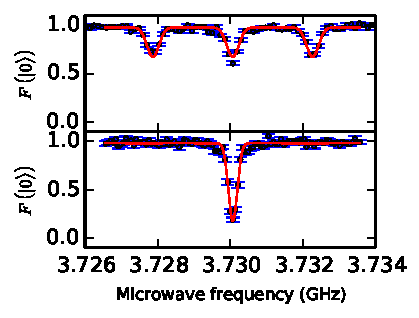
\includegraphics{Img/DarkESR_2.pdf}};
        \node (A) at (2.6,4.4) {};
        \node (B) at (3.92,4.4) { };
        \node (C) at (5.3,4.4) { };
        \draw[latex-latex, font=\small] (A) -- node[label =270: $A_\mathrm{N}$] {} (B);
        \draw[latex-latex, font=\small] (B) -- node[label =270: $A_\mathrm{N}$] {} (C);
    \end{tikzpicture}
    \caption{dark Electron Spin Resonance (ESR) for uninitialized (top) and initialized nitrogen spin (bottom) of the $m_s =0 \rightarrow m_s = +1$ transition. In a dark ESR the spin is prepared in $\ket{0}$, a microwave pulse is applied and then the $\ket{0}$ state is read-out again. This is done for a range of frequencies. When the microwave is on resonance with a transition the spin will be rotated and a dip will be visible in the signal. In the top figure the transition is split due to the interaction with the nearby nitrogen atom. In the lower figure the nitrogen state is initialized and the splitting disappears.}
    \label{fig:HF_split_levels}
\end{figure}

\subsection{Strongly-coupled spins}
An example of a strongly coupled spin is the NV-nitrogen spin.
The strength of the coupling between the nitrogen and the electronic spin is $A_\mathrm{N} = 2\pi \cdot 2.186\quad \mathrm{MHz} $\citep{Bernien2014Control} and it acts along the NV-axis.
\Cref{fig:HF_split_levels} clearly shows the $m_s =0 \rightarrow m_s=+1$ transitions being split due to hyperfine-coupling to the nitrogen.
This splitting can be used to control the nitrogen.
By first initializing in the $m_s =+1$-state and then applying a slow pulse that turns only one of the three nitrogen spin-states back to $m_s=0$ and reading out the nitrogen-spin can be initialized. By only continuing on a positive outcome the spin is initialized in the state that was rotated back to $m_s =0$. We call this measurement-based-initialization (MBI).
The lower panel of \cref{fig:HF_split_levels} shows a dark Electron-Spin-Resonance (ESR) after nitrogen-MBI.

In a similar way strongly-coupled carbon-13 atoms can be controlled\citep{Robledo2011HighFidelity}.
For most strongly-coupled carbons the contact term in the hyperfine is not negligible.
For these carbons hyperfine couplings have been measured\citep{Smeltzer201113} and calculated\citep{Gali2008Ab,Gali2009Identification}.

\subsection{Weakly-coupled carbon spins}
For carbons where the contact term is negligible the hyperfine-term is equal to the dipole term and is given by \cref{eq:dipole_component_of_hyperfine}\citep{Lange2012Quantum}.
With $n_\mathrm{HF}$ is a unit vector pointing from the NV-center to the nucleus and $r$ the distance between them.
$\mathbf{S}$ and $\mathbf{I}$are the spin operators for the NV-spin and the nucleus, $\gamma_e $ the gyromagnetic ratio of the electron, $\gamma_n$ the gyromagnetic ratio of the nucleus, and $\mu_0$ the magnetic permeability.
For weakly-coupled carbons the contact-term of the hyperfine is generally\footnote{Only under exceptionally high carbon-13 concentrations is $T_{2e}^*$ short enough for close by carbon-13 atoms to fall under the definition of weakly coupled. } negligible.

\begin{equation}
\label{eq:dipole_component_of_hyperfine}
H_{\mathrm{dip}} = \frac{\mu_0 \gamma_e \gamma_{\mathrm{C}} \hbar^2 }{4 \pi r^3} [ \bm{S \cdot I} - 3 (\bm S \cdot \hat{n_{\mathrm{hf}}})(\bm I \cdot \hat{n_{\mathrm{hf}}})]
\end{equation}

From \cref{eq:dipole_component_of_hyperfine}  the parallel and orthogonal components of the Hyperfine interaction, with respect to the NV-axis along the z-direction, can be derived to be:
 \begin{eqnarray}
A_\parallel= - \frac{\mu_0 \gamma_e \gamma_{\mathrm{C}} \hbar^2 }{4 \pi r^3} \left(3\cdot \frac{z^2}{r^2}-1\right)\\
 A_\perp =  -\frac{\mu_0 \gamma_e \gamma_{\mathrm{C}} \hbar^2 }{4 \pi r^3}\left( 3\cdot\frac{\sqrt{x^2+y^2}\cdot z}{r^2}\right)
\end{eqnarray}
Where $H_{\mathrm{HF}} = A_\parallel I_\mathrm{z} + A_\perp I_x $.

At first sight it seems impossible to control weakly coupled spins as their transitions are obscured by the spin-bath.
It is however possible to increase the coherence time of the electron, stabilizing the transitions, allowing more spins to be resolved.

\subsection{Extending electron coherence}
In a spin-echo experiment a Ramsey experiment is performed with a small difference. An additional $\pi$ pulse is applied in the middle of the experiment exactly between the $\pi/2$ pulses. This pulse effectively turns the nuclear-spin environment upside-down halfway trough the experiment, making the qausi-static-part of the dephasing during the first and the second part of the free evolution cancel each other out, substantially increasing coherence on short-timescales ($\tau \ll T_2 $)
\footnote{ $T_2$ is a measure for decoherence. It is similar to $T_2^*$ but does not include variations between experiments. $T_2$ is defined as the $1/e$ time of the decay of a spin-echo experiment.}.
On longer timescales the difference between the initial part of the evolution and the final part of the evolution becomes larger making the initial and final part no longer cancel each other out.

A natural way of extending the short timescale behavior of the spin-echo to longer timescales is by applying more $\pi$-pulses. This procedure known as dynamical-decoupling can dramatically improve coherence times by decoupling the central-spin from the environment\citep{Lange2010Universal}.

Although dynamical-decoupling improves the coherence of the central spin by decoupling from the environment, the central spin is also decoupled from other spins preventing direct two-qubit gates. It was demonstrated by \citet{Sar2012DecoherenceProtected} how to incorporate dynamical decoupling in a universal gate design by implementing Grover's algorithm.
Using this technique \citet{Taminiau2012Detection} used the extended coherence to detect and control weakly-coupled carbon spins, before implementing three-qubit quantum-error-correction (QEC) \citep{Taminiau2014Universal}.

As these experiments where performed with NV-centers at Room temperature they lack the option to do single-shot readout required to act on a measurement outcome\footnote{@Tim, I think this can be worded more concisely. Do you have any ideas?}. An essential feature for the parity measurements that form the basis of measurement-based QEC and surface codes.

\subsection{Dynamical decoupling spectroscopy}
As we cannot perform an ESR experiment while decoupling a different technique must be used to resolve and address additional spins.
In order to resolve additional spins we perform a dynamical decoupling spectroscopy, resulting in a fingerprint of the nuclear-spin environment\citep{Taminiau2012Detection}.

In a dynamical decoupling spectroscopy experiment the electron is prepared in the $|X\rangle = |0\rangle +|1\rangle$ state. It is subjected to a decoupling sequence consisting of N/2 blocks of the form {$\tau - \pi -2\tau-\pi-\tau$}, and concluded by measuring $\langle X\rangle $. The fingerprint is the result of many repetitions for a range of inter-pulse delays $2\tau$. $\pi$ is a $\pi$-pulse.

Part of a dynamical decoupling spectroscopy can be seen in \cref{fig:FP}. The spectroscopy was performed for N = 8, 16, 32 and 64 pulses. For N = 8, 16 and 32 pulses this was done between $\tau = 2 \mu \mathrm{s}$  and $72 \mu \mathrm{s}$ and for N = 64 this was done up to $\tau = 52 \mu \mathrm{s}$. A reference to the full spectroscopy can be found in \cref{chap:Fingerprint_data_appendix}.

\begin{figure}[htbp]

    \begin{subfigure}[t]{\textwidth}\centering
        \centering
        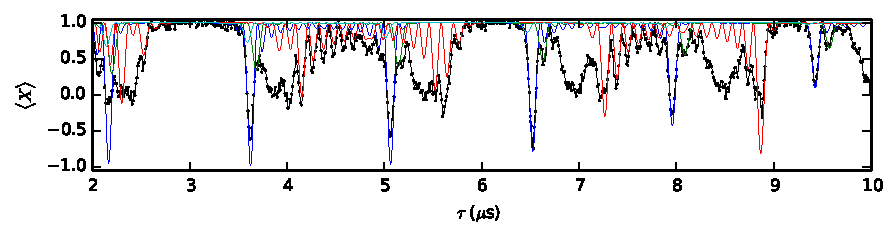
\includegraphics{Img/fingerprint16.pdf}
        %TODO_MAR: use annotations to add labels in the graphs using matplotlib
        \caption{Fingerprint for N=16 pulses. }
        \label{fig:FP16}
    \end{subfigure}

    \begin{subfigure}[t]{\textwidth}\centering
        \centering
        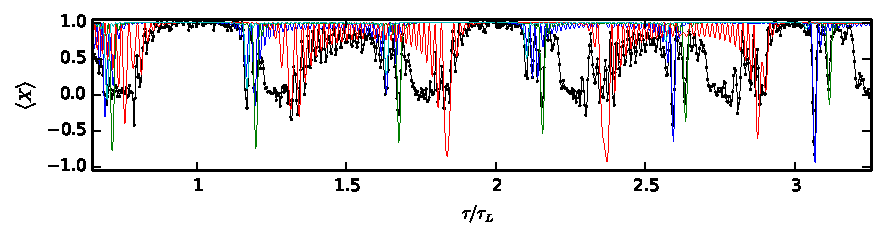
\includegraphics{Img/fingerprint32.pdf}
        %TODO_MAR: use annotations to add labels in the graphs using matplotlib
        \caption{Fingerprint for N =32 pulses. }
        \label{fig:FP32}
    \end{subfigure}
    \caption{Part of a fingerprint resulting from a dynamical-decoupling-spectroscopy experiment performed at 304.12G. A reference to the full spectroscopy can be found in \cref{chap:Fingerprint_data_appendix}.  Colored lines represent computed responses of carbon spins. Responses were calculated using \cref{eq:contrast_single_carbon_spin} with hyperfine parameters from \cref{tbl:HF_par}. }
    \label{fig:FP}
\end{figure}

\section{Addressing Weakly-coupled Carbons through Dynamical Decoupling}
\label{controllingacarbonthroughdynamicaldecoupling}

In order to understand how the features in the fingerprint from \cref{fig:FP} relate to the different spins and how this knowledge can be used to control these carbons it is necessary to understand what dynamical decoupling does to these atoms.

\subsection{The effect of dynamical decoupling}

\begin{figure}[htbp]
\centering
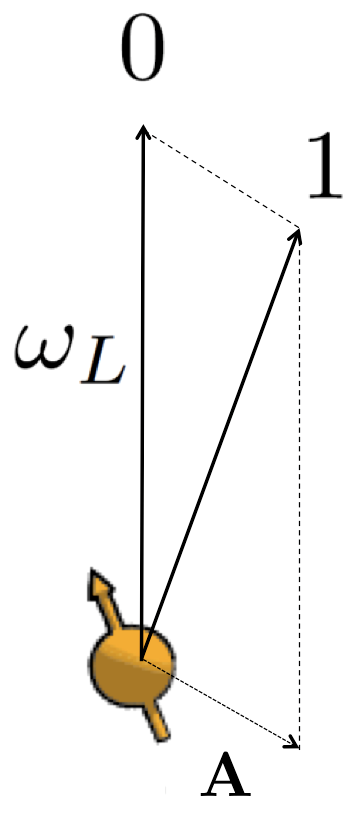
\includegraphics[keepaspectratio,width=0.15\textwidth]{./img/QuantizationAxis.png}
\caption{Flipping the electron spin from the  $m_s=0$ to the $m_s= +1$ state changes the quantization axis of nuclear spins. For  $m_s=0$ all nuclear spins precess about $\bm{\omega_L}$. For  $m_s=+1$ each spin precesses about a distinct axis $\bm{\tilde{\omega}}=\bm{\omega_L} +\bm{A}$.}
\label{fig:quantax}
\end{figure}

When the electron is in the $m_s=0$ state each nuclear spin precesses about $\bm{\omega_L}$ with the Larmor frequency. When the electron is in the $m_s=+1$ state nuclear spins precess about a distinct axis $\bm{\tilde{\omega}}=\bm{\omega_L} +\bm{A}$ \citep{Taminiau2012Detection}. The hyperfine interaction $\bm{A}$ depends on the position of that particular nuclear spin relative to the NV- center.

When applying a decoupling sequence with N\slash 2 decoupling units of the form {$\tau - \pi -2\tau-\pi-\tau$}, the nuclear spin alternately rotates around the  $\bm\omega_L$ and the $\bm{\tilde{\omega}}$ axis.
The net result of one such decoupling sequence is a rotation around an axis $\bm{\hat{\mathrm{n_i}}}$ by an angle $\phi$.
Where $\bm{\hat{\mathrm{n_i}}}$ depends on the initial state of the electron: $\bm{\hat{\mathrm{n_0}}}$ when the electron starts in $m_s = 0$ and $\bm{\hat{\mathrm{n_1}}}$ when the electron starts in $m_s = +1$~\citep{Taminiau2012Detection}.

\begin{figure}[htbp]
    \begin{subfigure}[t]{0.49\textwidth}\centering
        \centering
        \includegraphics{Img/unCond_rot_taminiau.pdf}
        \caption{Unconditional rotation.}
        \label{fig:uncond_rot}
    \end{subfigure}
    \begin{subfigure}[t]{0.49\textwidth}\centering
        \centering
        \includegraphics{Img/Cond_rot_taminiau.pdf}
        \caption{Conditional rotation.}
        \label{fig:cond_rot}
    \end{subfigure}
    \caption{\Cref{fig:uncond_rot} When the net rotation axes $\bm{\hat{\mathrm{n_0}}}$ and $\bm{\hat{\mathrm{n_1}}}$ point in the same direction the carbon experiences an unconditional rotation and cannot be controlled. \Cref{fig:cond_rot} When the net rotation axes $\bm{\hat{\mathrm{n_0}}}$ and $\bm{\hat{\mathrm{n_1}}}$ are anti-parallel the carbon experiences a conditional rotation, either around +x or -x, and can be controlled.}
    \label{fig:conditional_and_unconditional_rotation}
\end{figure}


To understand how a carbon-13 atom can be controlled it is useful to consider three situations. In the first situation the $\bm{\omega_L}$ and $\bm{A}$ point in the same direction. In the second situation $\bm{\omega_L}$ and $\bm{A_\perp}$ are of comparable magnitude, resulting in a large angle between the quantization axes. In the last situation $|\bm{A}|$ is small compared to  $\bm{|\omega_L|}$ resulting in a small angle between the quantization axes.

When $\bm{\omega_L}$ and $\bm{A}$ point in the same direction, the net rotation axis is independent of the initial electron-state making it impossible to use the electron to control the carbon-13 atom using this decoupling sequence.

In the case where $\bm{\omega_L}$ and $\bm{A_\perp}$ are of comparable magnitude the net rotation axes $\bm{\hat{\mathrm{n_i}}}$ are strongly dependent on the initial electron-state for almost any $\tau$. This creates entanglement between the electron and this carbon for a wide range of inter pulse-delays $\tau$. For future reference we say that these weakly-coupled carbons are in the \emph{complex regime}.

When considering the case where the hyperfine interaction is much smaller than the Larmor frequency ($\omega_L \gg |\bm{A}|$), the net rotation axes  $\hat{\mathrm{n_0}}$ and $\hat{\mathrm{n_1}}$ are practically parallel and the nuclear spin undergoes an unconditional evolution.
Only when the inter-pulse delay is precisely resonant with the spin dynamics the axes are anti-parallel leading to a conditional rotation\citep{Taminiau2012Detection}.
The resonant condition is given by \cref{eq:res_dip_loc}, where $k$ is an integer and the FWHM of the Lorentzian-shaped resonance is given by \cref{eq:res_dip_width}.
To distinguish these carbons from those in the complex regime we say that these weakly-coupled carbons are in the \emph{basic regime}.

% somehow state that resonance gives a dip.
 \begin{equation}
\tau = \frac{(2k+1)\pi}{2 \omega_L + A_\parallel}
\label{eq:res_dip_loc}
\end{equation}
 \begin{equation}
\Delta = \frac{A_\perp}{2 \omega_L^2}
\label{eq:res_dip_width}
\end{equation}

If  $\hat{n_0}$ and $\hat{n_1}$ are not parallel, the resulting conditional rotation of the nuclear spin generally entangles the electron and nuclear spins.

\subsection{Response of an isolated carbon to dynamical decoupling spectroscopy}

As a result the electronic spin, starting out in $\ket{X}$, entangles with the nuclear spin for specific values of $\tau$ during a dynamical decoupling spectroscopy.
When reading out the electronic spin along the X-axis this creates a dip in the signal.
The probability that the initial state is preserved is given by \cref{eq:contrast_to_probability}. Where the contrast $M_j$ for a single nuclear spin is given by \cref{eq:contrast_single_carbon_spin}\citep{Taminiau2012Detection}.

\begin{equation}
\label{eq:contrast_to_probability}
P_x = (M+1)/2
\end{equation}

\begin{equation}
\label{eq:contrast_single_carbon_spin}
M_j = 1-(1 - \hat{\bm{\mathrm{n_0}}} \cdot \hat{\bm{\mathrm{n_1}}}) \sin^2 \frac{N\phi}{2}
\end{equation}

%alpha = \tilde{\omega} \tau
%beta = (\omega_L \tau)
% mz = (\frac{ A_ \parallel + \omega_L }{ \tilde{ \omega}})
\begin{equation}
\label{eq:vec_term}
    1 - \hat{\bm{\mathrm{n_0}}} \cdot \hat{\bm{\mathrm{n_1}}} =  \frac{A_\perp ^2}{\tilde{\omega^2}} \frac{(1- \cos{(\tilde{\omega} \tau)})(1-\cos{(\omega_L \tau)})} {1 +\cos{(\tilde{\omega} \tau)}\cos{(\omega_L \tau)} - (\frac{ A_ \parallel + \omega_L }{ \tilde{ \omega}}) \sin{(\tilde{\omega} \tau)}\sin{(\omega_L \tau)}}
\end{equation}
\begin{equation}
\label{eq:angle_term}
    \phi =  \cos^{-1}\left(\cos(\tilde{\omega} \tau) \cos(\omega_L \tau)-\left(\frac{ A_ \parallel + \omega_L }{ \tilde{ \omega}}\right) \sin(\tilde{\omega} \tau)\sin(\omega_L \tau)\right)
\end{equation}

\subsection{Characterizing the Nuclear-spin environment}
% Should add some sort of introduction as to what is in this section

In reality the electron is not interacting with a single carbon but with a bath of carbon atoms. When the electron interacts with multiple carbons at the same time the contrast $M$ is given by the product of all individual values $M_j$ for each individual spin $j$ (\cref{eq:prod_multiple_spins}). In order to selectively control one carbon the electron should not entangle with any other carbon when addressing it.

\begin{equation}
\label{eq:prod_multiple_spins}
    M = \prod_{j}{M_j}
\end{equation}

When entanglement is created with multiple carbons at the same time coherence is quickly lost and contrast drops to 0.
By sweeping the number of pulses $\pi$-pules the response of an individual carbon can be distinguished from the response of multiple spins.
Only when an individual carbon is being addressed is it possible to sweep the contrast to -1.

% A narrow dip in the fingerprint spectrum is an indication of a selectively addressable carbon.
% By sweeping the number of $\pi$-pulses on such a dip it can be verified if it corresponds to a \emph{single} carbon.

Most spins are relatively far away from the NV-center and have similar hyperfine couplings causing their resonances to overlap. This causes a broad feature with low coherence known as the spin-bath collapse. This feature is clearly visible in the fingerprint (\cref{fig:FP}) at $\tau/(4\tau_L) = m$ for odd $m$, where $\tau_L$ is the Larmor period ($\tau_L = \frac{2\pi}{\omega_L} $).

Spins that have a stronger than average hyperfine-interaction show up outside or at the edge of the spin-bath collapse.
Spins that are in the basic regime show up as a narrow dip.
Going to larger $\tau$ separates these dips further as the order of the resonance $k$ increases.
By looking at larger $\tau$ it is possible to resolve and address more resonances.
Several spins in the basic regime have been identified 3 of these are visible as colored lines in \cref{fig:FP}.
As computations are fundamentally limited by the coherence time there is a limit to the resonance-order that can be used to address carbons, making it impossible to resolve all weakly coupled spins.

Besides the carbons in the basic regime there are also weakly-coupled carbons that are more strongly coupled.
When a carbon in the complex regime is present in the NV-center this manifests itself as a resonance with strong oscillations on the side. Such a feature is also clearly visible in \cref{fig:FP}. We have identified the oscillations in the fingerprint as belong to a single spin which is denoted by the red line.

When a weakly coupled carbon in the complex regime is present a significant part of the fingerprint spectrum is inaccessible for controlling other carbons making them an undesired feature when attempting to control weakly coupled carbon spins.


\subsection{Effect of the magnetic field}

There are significant advantages to increasing the magnetic field when attempting to address weakly coupled carbons.
By increasing the magnetic field the Larmor frequency can be increased, reducing the number of carbons that are in the complex regime.
This causes the broad oscillating resonances to disappear allowing more carbons to be addressed.

Although increasing the magnetic field can improve the situation it is not always possible or desired.
When the magnetic field becomes too strong too strong the resonances become narrower than the resolution of the Arbitrary Waveform Generator used to generate the pulses that address the resonances, making it impossible to address these resonances effectively.
Simulations were performed (see \cref{chap:addressable_carbon_sims}) that indicate that for a natural carbon-13 concentration there is a range between 400G and 1400G where the magnetic field is optimal for controlling weakly coupled spins.

Besides the spin environment there are other factors affecting the choice for magnetic field.
Because the optical transitions used for readout and initialization depend on strain and magnetic field field\citep{Hensen2011MeasurementBased}, care must be taken when measuring that states do not mix in the excited state.
This combined with the fact that few experiments have been performed at high magnetic field and low temperature make it more practical to settle for a more moderate magnetic field of 300G.

\subsection{Identifying Individual Carbon-spins}

We identify distinct features in the fingerprint, of which \cref{fig:FP} shows a small part,  and try to assign different hyperfine-couplings to them.
We then compute the response for these hyperfine couplings using \cref{eq:contrast_single_carbon_spin}.
The parameters are varied such that the computed response agrees with the data as well as possible.
Using this method 13 distinct carbon spins where identified.

The parameters of the 4 strongest coupled carbons are listed in \cref{tbl:HF_par} and their computed responses are visible as colored lines in \cref{fig:FP}.
All estimated hyperfine parameters and a link to the full fingerprint measurements can be found in \cref{chap:Fingerprint_data_appendix}.

\begin{table}[htbp]
    \begin{tabular}{cllll}
    Carbon & \quad \quad  $A_{\parallel} $ & \quad \quad $A_{\perp}$ \\ \hline
    1         & $2 \pi \cdot${ }30.0 kHz             & $2 \pi \cdot${ }80.0 kHz                \\
    2         & $2 \pi \cdot${ }27.0 kHz             & $2 \pi \cdot${ }28.5 kHz              \\
    3         & $2 \pi \cdot$-51.0 kHz          & $2 \pi \cdot$105.0 kHz              \\
    4         & $2 \pi \cdot${ }45.1 kHz           & $2 \pi \cdot${ }20.0 kHz                \\
    \end{tabular}
    \caption{Estimated hyperfine parameters for spins 1 to 4 in \cref{fig:FP}.}
    \label{tbl:HF_par}
\end{table}
 %split into subdocuments for the sections.


\chapter{Controlling Weakly-coupled Carbon Spins}
The creation of entanglement is an essential capability for QEC in particular and quantum-computation in general.
This chapter demonstrates how weakly coupled nuclear spins can be initialized and read-out and how this can be used to generate entanglement between them.
The creation of entanglement is demonstrated with a quantum state tomography.

\section{Initialization and readout of single spins}
\label{sec:carbon_init_and_readout}
A weakly coupled spin can be initialized by conditionalizing on a readout result, similar to how nitrogen-MBI works.
A weakly coupled carbon spin can be read-out by using the $\pm \mathrm{x}$-gate to entangle the phase of the electronic-spin with the state of the nuclear spin and reading out the phase of the electronic spin.

%Explain Readout.
The gates used to initialize a weakly coupled nuclear spin are depicted in \cref{fig:gate_circuit_initialization}.
The circuit depicted in \cref{fig:gate_circuit_mbi_x-init} is used to perform a read-out along the $x$-axis.
By applying a $\pm y$-gate on the carbon before the initial $y$-pulse the state can be read out along the $z$-axis.

%Explain Initialization.
\begin{figure}[htbp]
    \centering
    \begin{subfigure}[t]{0.49\textwidth}
    \centering
    \caption{}
    \mbox{
        \Qcircuit @C=1em @R=.7em {
        \lstick{\ket{0}_e}                        & \gate{\mathrm{y}}  & \ctrl{1}       & \gate{\mathrm{x}} &\qw          &  \meter \\
        \lstick{\rho_\mathrm{m}}         & \qw              &  \gate{\pm \mathrm{x}}     & \qw    & \qw   & \qw}}
    \label{fig:gate_circuit_mbi_x-init}
    \end{subfigure}
    \begin{subfigure}[t]{0.49\textwidth}
        \centering
        \caption{}
        \mbox{
        \Qcircuit @C=1em @R=.7em {
            \lstick{\ket{0}_e} & \gate{\mathrm{y}}  & \ctrl{1} & \gate{\mathrm{x}} &\ctrl{1} &  \meter \\
            \lstick{\rho_\mathrm{m}}& \qw&  \gate{\pm \mathrm{x}}     & \qw    & \gate{\mp \mathrm{y}}    & \qw}}
        \label{fig:gate_circuit_mbi_swap-init}
    \end{subfigure}
    \caption{\Cref{fig:gate_circuit_mbi_x-init} MBI-based initialization into $\pm \ket{\mathrm{X}}$. Initializes the carbon into $\ket{X}_\mathrm{C} $ when $\ket{0}_e$ is measured and into $\ket{-X}_\mathrm{C} $ when $\ket{1}_e$ is measured for the electron.
    \Cref{fig:gate_circuit_mbi_swap-init} MBI-swap initialization into $ \ket{\mathrm{0}}$. Initializes the carbon into $\ket{0}_\mathrm{C} $ regardless of the electronic spin-state measured.}
    \label{fig:gate_circuit_initialization}
\end{figure}


% To initialize the nuclear spin
The initial pulse in \cref{fig:gate_circuit_mbi_x-init} brings the electronic spin in $\ket{X}_e$.
When the nuclear spin starts in the mixed state the system can be described by the tensor product of two density matrices:
\begin{equation}
    \rho_X \otimes \rho_m = \rho_X \otimes \rho_{X} +\rho_X \otimes \rho_{-X}
\end{equation}
By applying the $\pm{\mathrm{x}}$-gate  the electronic-spin picks up a phase depending on the nuclear spin-state:
\begin{equation}
     \rho_Y \otimes \rho_{X} +\rho_{-Y} \otimes \rho_{-X}
\end{equation}
By reading out the electronic spin along the $y$-axis the nuclear spin is projected into the $\ket{X}_C$ or $\ket{-X}_C$-state.
By conditionalizing on a positive readout result the state can be initialized into the $\ket{X}_C$-state.

By adding a second conditional gate (\cref{fig:gate_circuit_mbi_swap-init}) the nuclear spin is brought into the $\ket{0}_C$-state regardless of the measurement outcome for the electronic spin.

\paragraph{}
\Cref{fig:single_qubit_initialization} demonstrates initialization and readout.
In \cref{fig:carbon_init_x} carbon-1 is initialized into the $\ket{X}_C$-state and in \cref{fig:carbon_init_Z} it is initialized into the $\ket{0}_C$-state.
This is done by implementing the circuits depicted in \cref{fig:gate_circuit_initialization} and conditionalizing on a positive electron readout.

The carbon is read out using the same circuits.
The blue points correspond to $x$-readout, the green points to $y$-readout and the red-points to the $z$-readout.
The phase is sweeped to demonstrate that the readouts function as intended.
For a qubit in the $\ket{0}$-state the initial phase is undefined.

The combined fidelity of readout and initialization to the desired state is: $F(\ket{X}) = 90.57 \pm 0.85 \% $ for the $\ket{X}$-state and $F(\ket{Z}) = 93.00 \pm 0.31 \%$ for the $\ket{Z}$-state.
% Add description of features if still have time after finished today :)

\begin{figure}[htbp]
    \begin{subfigure}[t]{0.49\textwidth}\centering
        \caption{}
        \includegraphics{Img/RO_and_init_C1_X.pdf}
        \label{fig:carbon_init_x}
    \end{subfigure}
        \begin{subfigure}[t]{0.49\textwidth}\centering
        \caption{}
        \includegraphics{Img/RO_and_init_C1_Z.pdf}
        \label{fig:carbon_init_Z}
    \end{subfigure}
    \caption{Demonstration of carbon initialization and readout. In \cref{fig:carbon_init_x} carbon-1 is initialized in $\ket{X}$ and read-out. In \cref{fig:carbon_init_Z} carbon-1 is initialized in $\ket{0}$. Colored points correspond to readouts in different bases, blue to $x$-readout, green to $y$-readout and red to $z$-readout.}
    \label{fig:single_qubit_initialization}
\end{figure}


\section{The parity measurement}
Entanglement between two qubits can be created by performing a parity measurement on them and conditionalizing on the outcome.

A parity measurement does not measure the state of two qubits but measures if  two qubits are the same in a certain basis.
An example is the XX-parity measurement.
The XX-parity measurement returns a positive result if the the two qubits are the same in the $x$-basis and a negative result if the two are opposite.
That is it returns a positive result if the state is $\ket{X,X}$ or $\ket{-X,-X}$ and a negative result if the state is $\ket{X,-X}$ or $\ket{-X,X}$.
In general a two qubit parity operator has 2 eigenvalues, both are twofold degenerate.

The XX-parity measurement can be implemented on a weakly coupled carbon spins using the circuit depicted in \cref{fig:gate_circuit_general_Parity_RO}.
A parity measurement is very similar to the regular readout depicted in \cref{fig:gate_circuit_mbi_x-init}.
Once the electron is brought into a superposition the electron picks up phase when the $\mp \mathrm{x}$-gate is applied.
$+\pi/2$-phase when the carbon is in $\ket{+X}$ and $-\pi/2$-phase when the carbon is in $\ket{-X}$.
This is done for both carbons, when both carbons are in the same $x$-state the electron will pick up $\pi$-phase.
When they do not give the same result the phase cancels.
By reading out the electronic-spin along $x$ the parity is measured.
It should be noted that because we use a $\pm \mathrm{x}$-gate instead of a CNOT-gate an additional $\pi/2$-phase is added to the carbon states compared to a regular parity measurement.

\begin{figure}[htbp]
    \centering
\mbox{
\Qcircuit @C=1em @R=.7em {
\lstick{\ket{0}_e} &  \gate{\mathrm{y}}  & \ctrl{1} &  \ctrl{2} & \gate{\mathrm{y}}  &  \meter &\qw\\
\lstick{\ket{\psi}_{C1}} &  \qw & \gate{\pm \mathrm{x}}  &\qw   &  \qw   &\qw&\qw \\
\lstick{\ket{\psi}_{C2}}   & \qw   & \qw    & \gate{\pm \mathrm{x}}   &\qw & \qw &\qw}}
    \caption{Gate circuit for a XX-parity measurement. }
    \label{fig:gate_circuit_general_Parity_RO}
\end{figure}

\section{Quantum state tomography}
To demonstrate entanglement, entanglement must not only be created but it must also be verified that the entangled state is created.
This can be done by performing a quantum state tomography.
In a quantum state tomography the density matrix of a quantum state is reconstructed by repeatedly preparing the same state and gathering measurement statistics in different bases.

An arbitrary matrix can be described as a weighted sum of the Pauli-matrices and the Identity as in: \cref{eq:pauli}.
\begin{equation}
    \rho = I + \sum_{i,j} a_{i,j} \sigma_i \otimes \sigma_j
    \label{eq:pauli}
\end{equation}
By measuring the coefficients of \cref{eq:pauli}  the density matrix $\rho$ can be reconstructed completely.


\subsection{Readout}
To measure the coefficients of \cref{eq:pauli} single and multi qubit measurements are needed.
Single qubit measurements were described in \cref{sec:carbon_init_and_readout}.
The two qubit measurements required are very similar to parity measurements but do not need to preserve the state after the measurement.

The parity measurement depicted in \cref{fig:gate_circuit_general_Parity_RO} can be used to measure the XX-parity.
By changing the phase of one or two of the two $\pm \mathrm{x}$ gates Y-parities can be measured.
By applying a $\mp \mathrm{y}$ to one of the two carbons before the initial Y-pulse a Z-parity can be measured, care must be taken however that the phase difference between this gate and the $\pm \mathrm{x}$ on the corresponding carbon is $90^\circ$.

% How readout is implemented
\subsection{Initialization and tomography of multiple weakly coupled spins}
Before entanglement can be created the system must be initialized.
We verify that we have correctly initialized the qubits by performing a tomography.
The results are compared to the expected coefficients for the ideal case.

\Cref{fig:uu-init } shows a tomography of carbon-1 and carbon-4 initialized in the $\ket{00}$-state.
In the ideal case the single qubit Z-measurements and the ZZ parity are 1 and all other coefficients are 0.
The ideal case is represented by the gray bars in the \cref{fig:uu-init }.
The fidelity to the ideal case is $F = 81.43 \pm 1.68$ \%.

\Cref{fig:ud-init } shows a tomography of carbon-1 and carbon-4 initialized in the $\ket{01}$-state.
In the ideal case ZI =1 and IZ and ZZ are -1, all other coefficients are 0.
The ideal case is represented by the gray bars in the \cref{fig:ud-init }.
The fidelity to the ideal case prediction is $80.99 \pm 1.69$ \%.

\begin{figure}[htbp]
    \begin{subfigure}[t]{0.49\textwidth}\centering
        \caption{}
        \includegraphics{Img/uu-no-parity.pdf}
        \label{fig:uu-init }
    \end{subfigure}
    \begin{subfigure}[t]{0.49\textwidth}\centering
        \caption{}
        \includegraphics{Img/ud-no-parity.pdf}
        \label{fig:ud-init }
    \end{subfigure}
    \caption{ Quantum state tomographies of two initialized carbons. In \cref{fig:uu-init } the carbons are initialized into $\ket{00}$ with a fidelity of  $81.43 \pm 1.68$ \%.
    In \cref{fig:ud-init } the carbons are initialized into $\ket{10}$ with a fidelity of $80.99 \pm 1.69$ \%.
    }
    \label{fig:2qubitTomos}
\end{figure}

\section{Demonstrating entanglement between weakly coupled carbons}
Now that we are able to initialize multiple weakly coupled carbon spins and verify this with a tomography it is possible to demonstrate entanglement.
After the qubits are initialized an XX-parity is performed and the tomography is conditionalized on the negative readout result.

By conditionalizing on the negative readout result the carbons are projected into the negative-parity eigenstates of the XX-parity operator.
These are $\ket{-X,X}$ and $\ket{-X,X}$.
The tomography coefficient for the XX-parity is trivially -1.
The other coefficients depend on the initial state the parity was performed on.
The expected coefficients can be found as the expectation values of the operators on the state: $\bra{\Psi} \sigma_i \otimes \sigma_j \ket{\Psi}$ and are again depicted as gray bars.

\Cref{fig:uu-XX} shows the tomography for the negative XX parity of the $\ket{00}$-state.
$\ket{00}$ can be written in the X-basis as:
\begin{equation}
      \tfrac{1}{2} \left( \ket{X,X} + \ket{X,-X} +\ket{X,-X} + \ket{-X,-X} \right)
 \end{equation}
By measuring the negative XX-parity the state is projected onto:
\begin{equation}
    \tfrac{1}{\sqrt{2}} \left( \ket{X,-X} +\ket{X,-X} \right)
\end{equation}
The expectation for the ideal case is represented by the gray bars.
The fidelity to the ideal case prediction is $76.60 \pm 1.74$ \%.

\paragraph{ }
\Cref{fig:ud-XX} shows the tomography for the negative XX parity of the $\ket{01}$-state.
$\ket{01}$ can be written in the X-basis as:
\begin{equation}
    \tfrac{1}{2} \left( \ket{X,X} - \ket{X,-X} +\ket{X,-X} - \ket{-X,-X} \right)
 \end{equation}
By measuring the negative XX-parity the state is projected onto:
\begin{equation}
    \tfrac{1}{\sqrt{2}} \left( \ket{X,-X} -\ket{X,-X} \right)
\end{equation}
The expectation for the ideal case is represented by the gray bars.
The fidelity to the ideal case prediction is  $76.08 \pm 1.74$ \%


\begin{figure}[htbp]
    \begin{subfigure}[t]{0.49\textwidth}\centering
        \caption{}
        \includegraphics{Img/uu-XX-parity.pdf}
        \label{fig:uu-XX}
    \end{subfigure}
    \begin{subfigure}[t]{0.49\textwidth}\centering
        \caption{}
        \includegraphics{Img/ud-XX-parity.pdf}
        \label{fig:ud-XX}
    \end{subfigure}
    \caption{ Quantum state tomographies for entangled states created by measuring a negative XX parity.
    \Cref{fig:uu-XX} is the negative XX-parity of the state prepared in \cref{fig:uu-init }. It is in the $    \tfrac{1}{\sqrt{2}} \left( \ket{X,-X} +\ket{X,-X} \right)
$ with  $76.60 \pm 1.74\%$ fidelity.
    \Cref{fig:ud-XX} is the negative XX-parity of the state prepared in \cref{fig:ud-init }. It is in the $\tfrac{1}{\sqrt{2}} \left( \ket{X,-X} -\ket{X,-X} \right)$  with  $76.08 \pm 1.74$ \% fidelity.
    }
    \label{fig:2qubit_parity_Tomos}
\end{figure}

Some conclusion...


% Consists of several sub chapters
    %  theory of how weakly coupled carbons can be controlled
    %  Experiments used to characterize the environment and carbons
    %  Theory of initialization and readout of carbons
    %  Experiments showing single and multiple carbon initialization and readout
% \chapter{Deterministic Parity Measurements}


\section{Entanglement}
%  Section gives definition of entanglement and refers to appendix for derivation of entanglement wittness.

\section{Verification of Entanglement}
% Section gives Results hopefully showing F>0.5 to Bell state with a cheer
%  Don't forget to elaborate where the error bars come from; statistical and does not include gate errors

%  Entanglement verification as test to check both feed forward and parity measurements
% Experiment (hopefully) showing F>0.5 to Bell state.
\chapter{Towards Quantum Error Correction}
Two more challenges remain to realize quantum error correction based on the parity measurements demonstrated in \cref{chap:control_weakly_carbon}.
First, to correct errors, gate operations that are conditional on the parity outcome are required.
Therefore the parity measurement must be accurate and preserve entangled state for both outcomes, unlike the probabilistic initialization and entanglement in this thesis.

Second, for error correction encoding in larger entangled states is required: at least three qubits for the simplest error correction and at least five qubits for correction of all types of errors.
In this chapter I address these two challenges and present simulations that indicate that multi-qubit parity measurements on weakly coupled spins are possible.

\section{Deterministic Parity Measurements}

An essential capability for QEC is the ability to perform different quantum operations based on a classical readout result.
An example of such an experiment is the deterministic creation of entanglement, as was demonstrated by \citet{Riste2013Deterministic} in a different system.

By applying an extra set of gates when the negative result is measured in a parity measurement the state can be transformed in the state that would have been created had the positive parity been measured.
This capability is particular important for QEC where the result of a parity measurement determines whether a correcting gate must be applied.

The main challenge when performing such operations is to keep track of the phase of the system while waiting for the readout result that determines which set of gates should be executed.
The measurement environment developed for the work in this thesis automatically keep track of phases and has been set up to be extendable and compatible with such feed forward capabilities.

%Several challenges -> extra phase, Keeping track of things
% An additional advantage of performing deterministic operations is that it can significantly speed up the rate at which experiments can be performed as it is no longer limited by part of the probabilistic initialization.


\section{Multi Qubit Control}
In order to implement QEC more than the two qubits that were addressed must be addressed.
To correct for a single type of quantum error 3 qubits are required.
To correct for any type of quantum error at least 5 qubits are required.


\subsection{Working of the simulations}
Simulations were performed to determine how many weakly coupled carbons can be controlled, on average, for an NV-center using dynamical decoupling.
In the simulations statistics were collected on 1000 NV-centers for a range of magnetic fields and three different carbon-13 concentrations.
%HOW MANY FOR EACH
For all NV-centers an environment of carbon-13 spins randomly placed on lattice points was generated.
For lower concentrations a larger environment was simulated such that the total number of simulated carbon spins was $\sim 300$ per NV-center for all concentrations.

NV-centers containing a carbon with a hyperfine coupling larger than $200\,\mathrm{kHz}$ were rejected as such spins are prone to decohere during the optical readout of the electron spin and their complex dynamics at moderate field complicate spin control of other spins (\cref{chap:addressing_weakly_coupled_carbons}).
In an experimental setting these carbons can be easily detected and the NV-centers rejected.

On the remaining centers the hyperfine coupling between each carbon and the NV-center as well as the resonance conditions of these carbons were calculated.
% 299 for \mu = 1.1%, 423 for 0.33% and even more for 0.011% (data loading crashes..).
At these resonances it was determined if a carbon can be selectively and coherently controlled.

%Definition addressable
As a figure of merit we take the fidelity $F$ of the electron spin after two consecutive $\pm \mathrm{x}$ gates.
The first gate entangles the electron spin with the nuclear spin and the second gate disentangles the two.
Reduced electron spin fidelity indicates gate imperfections or unwanted entanglement of the electron to the other carbon-13 spins.
The threshold for a carbon-13 to be considered controllable is set at $F = 90 \, \%$.

The fidelity is determined by sweeping the number of pulses at the resonance conditions and determining with what fidelity two consecutive $\pm \mathrm{x}$-gates can be implemented.
The accuracy with which the resonance can be addressed is limited by the resolution of the arbitrary waveform generator at $1\,\mathrm{ns}$.
The fidelity is determined under the assumption of perfect $\pi$ and $\pi/2$ pulses on the electron.

%Decoherence implemented
Additionally we require to be able to perform 10 such gates within the coherence time.
For simplicity we do not simulate the nuclear-nuclear interactions and instead set $T_2^*$ as in \cref{tbl:concentration_Tmaxes}.
% interpulse delay.
Finally, we set a maximum value for the inter pulse delay $\tau_{\mathrm{max}}$, to take into account the limited coherence for the electron at large $\tau$.
$\tau_{\mathrm{max}}$ is set at the values listed in \cref{tbl:concentration_Tmaxes}.
%Table listing times used
\begin{table}[htbp]
    \centering
    \caption{Coherence times and maximum resonance time as used in the simulations.}
    \begin{tabular}{ccc}
    Concentration &  $  T_{2,C}^* $ & $  \tau_{\mathrm{max} }$ \\ \hline
    $1.10\,\% $&  7ms & $10\,\mu\mathrm{s}$\\
    $0.33\,\% $&  45ms & $36.7\,\mu\mathrm{s}$\\
    $0.11\,\% $&  70ms & $100\,\mu\mathrm{s}$\\
    \end{tabular}
    \label{tbl:concentration_Tmaxes}
\end{table}

\subsection{Results of the simulation}
\Cref{fig:Simulations_avg_n_vs_bfield} shows the average number of addressable carbon spins as a function of magnetic field.
The number of addressable carbons increases quickly at first before a slow decay sets in.

The initial increase in the number of addressable carbons can be explained by the Larmor frequency becoming larger than the hyperfine interaction.
At low magnetic field ($\omega_L \sim A$) most spins undergo complex dynamics.
When the Larmor frequency becomes larger than the hyperfine coupling of a carbon spin it is in the simple regime where the resonances are narrow.
Because there is less overlap more spins can be addressed.
This increase drops off because eventually all spins are in the simple regime.

By increasing the magnetic field further the resonances both get narrower (\cref{eq:res_dip_width}) and move to shorter times \cref{eq:res_dip_loc}.
When the field becomes too high a resonance can become too narrow to accurately address.
This is limited by the 1ns timing resolution of the arbitrary waveform generator.
Therefore the number of addressable spins decreases at high fields.

For lower concentrations there are on average less spins undergoing complex dynamics for the same magnetic field.
This causes the initial increase in addressable carbons to be steeper at lower concentrations.

There is also a bias due to the rejection of carbons with $|A|>200\,\mathrm{kHz}$.
Not rejecting these carbons will lower the number of addressable carbons for low magnetic fields as the response of these carbons dominates the dynamical decoupling spectroscopy, while the number of addressable carbons will increase slightly in the high field limit were these carbons can be controlled trough dynamical decoupling.

\begin{figure}[htbp]
    \begin{subfigure}[t]{0.49\textwidth}\centering
        \caption{}
        \begin{tikzpicture}
            \node[anchor=south west,inner sep=0] at (0,0) {\includegraphics{Img/Simulations_avgN_vs_Bfield.pdf}};
            \node[font=\small, text = blue] at (5.0,4.90)  {$\mu = 1.10\,\%$};
            \node[font=\small, text = green] at (5.0,4.6)  {$\mu =0.33\,\%$};
            \node[font=\small, text = red] at (5.0,4.30)  {$\mu =0.11\,\%$};
        \end{tikzpicture}
        \label{fig:Simulations_avg_n_vs_bfield}
    \end{subfigure}
    \begin{subfigure}[t]{0.49\textwidth}\centering
    \caption{}
    \begin{tikzpicture}
        \node[anchor=south west,inner sep=0] at (0,0) {\includegraphics{Img/Simulations_Histogram_vs_Bfield.pdf}};
        \node[font=\small, text = black] at (5.4,4.90)  {$B = 700\,\mathrm{G}$};
        \node[font=\small, text = black] at (5.4,4.60)  {$\mu = 1.1\,\%$};
    \end{tikzpicture}
    \label{fig:simulations_histogram_vs_Bfield}
    \end{subfigure}
    \caption{Simulation results calculating the number of addressable carbons in NV-centers containing no carbons with hyperfine coupling larger than $200\mathrm{kHz}$. \subref{fig:Simulations_avg_n_vs_bfield} Average number of addressable carbons at different concentrations. \subref{fig:simulations_histogram_vs_Bfield} Normalized occurrences for $\mu = 1.1\,\%$ at $700\,\mathrm{G}$. The simulation indicates that an NV-center likely has 3 or more addressable carbons($P=89\,\%$), that there is a good chance that 5 or more carbons can be addressed ($P=57\,\%$) and that there is even a small probability of getting $\sim 10$ addressable carbon spins. }
    \label{fig:Simulation_results}
\end{figure}



% LONGER COHERENCE TIME
% When the concentration is lower the average separation between carbons and between carbons and the NV- centre is larger. This means that the coherence times are longer and that the coupling between a carbon and the NV- centre is on average weaker.

% OVERLAP
% One would expect that having less carbon atoms means less overlap in the resonances. Having less carbons might mean losing an easy to address carbon that is located close by. This effect is countered by also having some relatively weakly coupled carbons removed reducing overlap in resonances. The exact balance between these two effects depends on the configuration of each individual NV- centre.

% LONGER GATE TIMES
% Because the carbon atoms are coupled more weakly the magnetic field that is required before they can be resonantly addressed is much smaller. The downside of the weaker coupling is that the time it takes to implement a gate is much larger. Longer coherence times allow for longer gate times.

% LONGER RES TIME ALLOWED
% Because the longer coherence time a longer inter-pulse delay is allowed. This allows higher order peaks to be addressed at low magnetic fields. This allows additional carbon atoms to be controlled at low magnetic fields.

% DECLINE
% Eventually the dips become too narrow to address with the AWG. Because the width of the dips (\autoref{eq:res_dip_width}) depends on the strength of the coupling we expect this decline to set in earlier for lower concentrations as the carbons that are addressed are on average weaker coupled.


\paragraph{ }
\Cref{fig:simulations_histogram_vs_Bfield} shows the distribution of addressable carbons for a natural concentration of carbon-13 at the magnetic field that has the highest average number of addressable carbons.
It indicates that in most NV-centers ($89\,\%$) three or more carbons can be addressed and that in a reasonable fraction ($57\,\%$) of the samples five or more carbons can be addressed.
There are even rare occurrences where ten or more carbons can be addressed.

% % %%%%%%%%%
% Idem:

% Spins that have a stronger than average hyperfine-interaction show up outside or at the edge of the spin-bath collapse.
% Spins that are in the basic regime show up as a narrow dip.
% Going to larger $\tau$ separates these dips further as the order of the resonance $k$ increases.
% By looking at larger $\tau$ it is possible to resolve and address more resonances.
% Several spins in the basic regime have been identified 3 of these are visible as colored lines in \cref{fig:FP}.
% As computations are fundamentally limited by the coherence time there is a limit to the resonance-order that can be used to address carbons, making it impossible to resolve all weakly coupled spins.

% Besides the carbons in the basic regime there are also weakly-coupled carbons that are more strongly coupled.
% When a carbon in the complex regime is present in the NV-center this manifests itself as a resonance with strong oscillations on the side. Such a feature is also clearly visible in \cref{fig:FP}. We have identified the oscillations in the fingerprint as belong to a single spin which is denoted by the red line.

% When a weakly coupled carbon in the complex regime is present a significant part of the fingerprint spectrum is inaccessible for controlling other carbons making them an undesired feature when attempting to control weakly coupled carbon spins.



% Moved from identification section:
% \subsection{Effect of the magnetic field}

% Although increasing the magnetic field can improve the situation it is not always possible or desired.
% When the magnetic field becomes too strong too strong the resonances become narrower than the resolution of the Arbitrary Waveform Generator used to generate the pulses that address the resonances, making it impossible to address these resonances effectively.
% Simulations were performed (see \cref{chap:addressable_carbon_sims}) that indicate that for a natural carbon-13 concentration there is a range between 400G and 1400G where the magnetic field is optimal for controlling weakly coupled spins.

% Besides the spin environment there are other factors affecting the choice for magnetic field.
% Because the optical transitions used for readout and initialization depend on strain and magnetic field field\citep{Hensen2011MeasurementBased}, care must be taken when measuring that states do not mix in the excited state.
% This combined with the fact that few experiments have been performed at high magnetic field and low temperature make it more practical to settle for a more moderate magnetic field of 300G.

%  Outlook what more is needed for QEC
%  Short term outlook that indicates usefull 3 qubit QEC circuits
% Simulations showing long term outlook for quantum nodes


%%% FINAL stuff
\bibliographystyle{plainnat}
\bibliography{Remote}
\addcontentsline{toc}{chapter}{Bibliography}

%%% appendices
%Note all data analysis figures are saved in an ipython notebook saved in the analysis/LT2/Master Thesis Figures Adriaan.ipynb and uses only scripts that can be found in the analysis folder in sublime.

\appendix
%Appendix that explicitly calculates what states you get and how the gates work
\chapter{Dynamical Decoupling Spectroscopy}

\section{Mathematical description of dynamical decoupling spectroscopy}
\label{sec:mathematical_description_dd_spectro}


The response of a single carbon to a dynamical decoupling spectroscopy experiment is given by \cref{eq:contrast_to_probability,eq:contrast_single_carbon_spin,eq:vec_term,eq:angle_term} \citep{Taminiau2012Detection}. Where $P_x$ is the probability that the initial spin-state is preserved and $M_j$ the contrast.
\begin{equation}
\label{eq:contrast_to_probability}
P_x = (M+1)/2
\end{equation}

\begin{equation}
\label{eq:contrast_single_carbon_spin}
M_j = 1-(1 - \hat{\bm{\mathrm{n_0}}} \cdot \hat{\bm{\mathrm{n_1}}}) \sin^2 \frac{N\phi}{2}
\end{equation}

%alpha = \tilde{\omega} \tau
%beta = (\omega_L \tau)
% mz = (\frac{ A_ \parallel + \omega_L }{ \tilde{ \omega}})
\begin{equation}
\label{eq:vec_term}
    1 - \hat{\bm{\mathrm{n_0}}} \cdot \hat{\bm{\mathrm{n_1}}} =  \frac{A_\perp ^2}{\tilde{\omega^2}} \frac{(1- \cos{(\tilde{\omega} \tau)})(1-\cos{(\omega_L \tau)})} {1 +\cos{(\tilde{\omega} \tau)}\cos{(\omega_L \tau)} - (\frac{ A_ \parallel + \omega_L }{ \tilde{ \omega}}) \sin{(\tilde{\omega} \tau)}\sin{(\omega_L \tau)}}
\end{equation}
\begin{equation}
\label{eq:angle_term}
    \phi =  \cos^{-1}\left(\cos(\tilde{\omega} \tau) \cos(\omega_L \tau)-\left(\frac{ A_ \parallel + \omega_L }{ \tilde{ \omega}}\right) \sin(\tilde{\omega} \tau)\sin(\omega_L \tau)\right)
\end{equation}

The contrast of an ensemble of spins in a dynamical decoupling spectroscopy$M$ is given by the product of all individual values $M_j$ for each individual spin $j$ (\cref{eq:app_prod_multiple_spins}).

\begin{equation}
    M = \prod_{j}{M_j}
    \label{eq:app_prod_multiple_spins}
\end{equation}


\section{Fingerprint analysis}
\label{chap:Fingerprint_data_appendix}
The estimated hyperfine paramters of all 13 identified spins can be found in \cref{tbl:HF_par_appendix}. Due to the size of the fingerprint analysis it is not possible to include with this thesis. A pdf file containing the fingerprint analysis can be found here: \url{https://www.dropbox.com/s/gieji9e86bfvsf1/fingerprinting.pdf}.

\begin{table}[htbp]
    \centering
    \caption{Estimated hyperfine parameters for spins 1 to 13.}
    \begin{tabular}{cllll}
    Carbon &  $\quad \quad A_{\parallel} $ &\quad \quad  $A_{\perp}$ \\ \hline
    1 & 2$\pi \cdot ${ }30.0 kHz & 2$\pi \cdot ${ }80.0 kHz \\
    2 & 2$\pi \cdot ${ }27.0 kHz & 2$\pi \cdot ${ }28.5 kHz \\
    3 & 2$\pi \cdot $-51.0 kHz & 2$\pi \cdot $105.0 kHz \\
    4 & 2$\pi \cdot ${ }45.1 kHz & 2$\pi \cdot ${ }20.0 kHz \\
    5 & 2$\pi \cdot ${ }17.0 kHz & 2$\pi \cdot ${ }10.0 kHz \\
    6 & 2$\pi \cdot $-15.0 kHz & 2$\pi \cdot ${ }12.0 kHz \\
    7 & 2$\pi \cdot $-23.0 kHz & 2$\pi \cdot ${ }12.0 kHz \\
    8 & 2$\pi \cdot ${ }10.0 kHz & 2$\pi \cdot ${ }{ }8.0 kHz \\
    9 & 2$\pi \cdot ${ }{ }8.0 kHz & 2$\pi \cdot ${ }12.0 kHz \\
    10 & 2$\pi \cdot ${ }-9.3 kHz & 2$\pi \cdot ${ }13.0 kHz \\
    11 & 2$\pi \cdot $-10.0 kHz & 2$\pi \cdot ${ }{ }5.0 kHz \\
    12 & 2$\pi \cdot $-30.0 kHz & 2$\pi \cdot ${ }35.0 kHz \\
    13 & 2$\pi \cdot $-32.0 kHz & 2$\pi \cdot ${ }20.0 kHz \\
    \end{tabular}
    \label{tbl:HF_par_appendix}
\end{table}

% \input{Nuclear_initialization.tex} Algebra for initializing a nuclear spin state in X or 0 using swap or mbi
% \chapter{State Initialization}

%Derivation of the operation the gate circuit does and how it initializes

% Same for the Tomography/Readout

% Appendix that calculates what the tomography results will be for the different Bell states
% \chapter{Bell State Tomography}
Derivation, what would a tomography of the Psi+ state look like?

% Appendix that performs derivation of entanglement wittness
% \chapter{Entanglement wittness}
% Derivation of F>0.5 to Bell state as entanglement wittness

%Appendix showing how the simulations work and some more details about it.
% \chapter{Simulations and Calculations for Number of Addressable Carbons}
\label{chap:addressable_carbon_sims}

\section{Scaling of number of resonances with magnetic field}
Starting from \cref{eq:res_dip_loc}

\begin{equation}
    \tau = \frac{(2k+1)\pi}{2\omega_L+A_\parallel}
\end{equation}
In the limit where $\bm{\omega_L} \gg \bm{A}$ the number of resonances $K$ of a single carbon between $\tau = 0$ and $\tau = T_{\mathrm{DD},e}$ scales linear with the magnetic field: $N_k \propto \omega_L$.

At the same time the width of these resonances decreases quadratically with magnetic field (\cref{eq:res_dip_width}).
\begin{equation}
    \Delta = \frac{A_\perp }{2\omega_L^2}
\end{equation}
Combining these two we find that the number of resonances $N$ that fit between two orders to increase linearly with magnetic field.
\begin{align}
N_k -N_{k-1} = \frac{\tau_{k+1} -\tau_k} {\Delta} \\
N_k -N_{k-1} = \frac{2\pi}{2\omega_L +A_\parallel} \cdot \frac{2\omega_L ^2}{A\perp}\\
N_k -N_{k-1} = \frac{2\pi \omega_L}{A_\perp }
\end{align}



Meanwhile the time it takes to implement a $\pi/2$-gate is given by \cref{eq:number_of_pulses} where $N_{\pi/2} $ is the number of pulses required for a $\pi/2$-pulse.
\begin{equation}
    T_{\pi/2}= N_{\pi/2} \tau
    \label{eq:number_of_pulses}
\end{equation}
Using \cref{eq:contrast_single_carbon_spin}, and noting that $\hat{\mathrm{n_0}}$ and $\hat{\mathrm{n_1}}$ are anti-parallel at the resonance condition, we can find N to be:
\begin{align}
    \frac{\pi}{4} = \frac{N_{\pi/2} \phi}{2}\\
    N_{\pi/2}=\frac{\pi}{2\phi}
\end{align}
Where $\phi$ is given by \cref{eq:angle_term}.
\begin{equation}
    \phi =  \cos^{-1}\left(\cos(\tilde{\omega} \tau) \cos(\omega_L \tau)-\left(\frac{ A_ \parallel + \omega_L }{ \tilde{ \omega}}\right) \sin(\tilde{\omega} \tau)\sin(\omega_L \tau)\right)
    \label{eq:angle_term_appendix}
\end{equation}
In the limit where $\bm{\omega_L} \gg \bm{A}$, $\omega_L \approx \tilde{\omega}$ simplifying \cref{eq:angle_term_appendix} to:
\begin{align}
    \phi = \cos^{-1} \left(\cos^2(\omega_L \tau) -  \sin^2(\omega_L \tau) \right)\\
    \phi = \cos^{-1} \left(2 \cos(\omega_L \tau)\right)
\end{align}
% Reinserting this in \cref{eq:number_of_pulses} we find
% \begin{align}
%     T_{\pi/2} = \left(\frac{\pi}{2 \omega_L \tau}\right) \tau \\
%     T_{\pi/2} = \frac{\pi}{2 \omega_L}\\
% \end{align}
% Leading to the surprising conclusion that operations become faster when increasing magnetic field in the limit of


\chapter{Constants and Experimental values}


\begin{table}[htbp]
    \begin{tabular}{cl}
    Constants  \\ \hline
    $\mu_0$&$4\pi \cdot 10^{-7 }\mathrm{\frac{V \cdot s}{A\cdot m}}$\\
    Gyromagnetic Ratios  \\ \hline
    $\gamma_e $ & $2\pi \cdot 2.8025\quad \mathrm{MHz/G} $ \\
    $\gamma_{N}$ & $2\pi \cdot 0.3077\quad \mathrm{kHz/G}$   \\
    $\gamma_\mathrm{C}$ & $2\pi \cdot 1.0705\quad \mathrm{kHz/G}$   \\ \hline
    \\
    Interaction Strengths  \\ \hline
    $\Delta $ & $2\pi \cdot 2.878\quad \mathrm{GHz} $\\
    $Q $ & $2\pi \cdot 4.946\quad \mathrm{MHz} $\\
    $A_N $ & $2\pi \cdot 2.186\quad \mathrm{MHz} $\\ \hline
    \\
    Optics\\ \hline
    637 nm & 471 THz \\ \hline
    \end{tabular}
    \label{tbl:constants and experimental values}
\end{table}


%%% ACKNOWLEDGEMENTS
% \chapter*{Acknowledgements}

% Tim for the immensely usefull feedback on my drafts, His interesting and for me new perspectives on what we are doing. Great coaching

% Julia.
% Ronald trust


\end{document}
